\documentclass{article}\usepackage[]{graphicx}\usepackage[]{xcolor}
% maxwidth is the original width if it is less than linewidth
% otherwise use linewidth (to make sure the graphics do not exceed the margin)
\makeatletter
\def\maxwidth{ %
  \ifdim\Gin@nat@width>\linewidth
    \linewidth
  \else
    \Gin@nat@width
  \fi
}
\makeatother

\definecolor{fgcolor}{rgb}{0.345, 0.345, 0.345}
\newcommand{\hlnum}[1]{\textcolor[rgb]{0.686,0.059,0.569}{#1}}%
\newcommand{\hlstr}[1]{\textcolor[rgb]{0.192,0.494,0.8}{#1}}%
\newcommand{\hlcom}[1]{\textcolor[rgb]{0.678,0.584,0.686}{\textit{#1}}}%
\newcommand{\hlopt}[1]{\textcolor[rgb]{0,0,0}{#1}}%
\newcommand{\hlstd}[1]{\textcolor[rgb]{0.345,0.345,0.345}{#1}}%
\newcommand{\hlkwa}[1]{\textcolor[rgb]{0.161,0.373,0.58}{\textbf{#1}}}%
\newcommand{\hlkwb}[1]{\textcolor[rgb]{0.69,0.353,0.396}{#1}}%
\newcommand{\hlkwc}[1]{\textcolor[rgb]{0.333,0.667,0.333}{#1}}%
\newcommand{\hlkwd}[1]{\textcolor[rgb]{0.737,0.353,0.396}{\textbf{#1}}}%
\let\hlipl\hlkwb

\usepackage{framed}
\makeatletter
\newenvironment{kframe}{%
 \def\at@end@of@kframe{}%
 \ifinner\ifhmode%
  \def\at@end@of@kframe{\end{minipage}}%
  \begin{minipage}{\columnwidth}%
 \fi\fi%
 \def\FrameCommand##1{\hskip\@totalleftmargin \hskip-\fboxsep
 \colorbox{shadecolor}{##1}\hskip-\fboxsep
     % There is no \\@totalrightmargin, so:
     \hskip-\linewidth \hskip-\@totalleftmargin \hskip\columnwidth}%
 \MakeFramed {\advance\hsize-\width
   \@totalleftmargin\z@ \linewidth\hsize
   \@setminipage}}%
 {\par\unskip\endMakeFramed%
 \at@end@of@kframe}
\makeatother

\definecolor{shadecolor}{rgb}{.97, .97, .97}
\definecolor{messagecolor}{rgb}{0, 0, 0}
\definecolor{warningcolor}{rgb}{1, 0, 1}
\definecolor{errorcolor}{rgb}{1, 0, 0}
\newenvironment{knitrout}{}{} % an empty environment to be redefined in TeX

\usepackage{alltt}
%Comments -- anything after % is not put into the PDF
\usepackage{amsmath} %This allows me to use the align functionality.
                     %If you find yourself trying to replicate
                     %something you found online, ensure you're
                     %loading the necessary packages!
\usepackage{amsfonts}%Math font
\usepackage{graphicx}%For including graphics
\usepackage{hyperref}%For Hyperlinks
\usepackage{natbib}%For the bibliography
\usepackage{parskip}%removes indents
\usepackage{color}%For colors
\usepackage{paralist}
\usepackage{enumerate}%allows us to make lists of items
\bibliographystyle{apalike}%For the bibliography
\usepackage[margin=0.80in]{geometry}%A way to change the length and layout of different elements
\usepackage{float}%Improves the interface for defining floating objects such as figures and tables. 
\newtheorem{definition}{Definition}[section]
\IfFileExists{upquote.sty}{\usepackage{upquote}}{}
\begin{document}

\begin{center}
\textbf{MTH-245 Final project Part 2} \\
\textbf{Fall 2022}\\
\end{center}

\vspace{.3cm}

\textbf{Name: } 

\vspace{.3cm}

\begin{knitrout}
\definecolor{shadecolor}{rgb}{0.969, 0.969, 0.969}\color{fgcolor}\begin{kframe}
\begin{alltt}
\hlkwd{library}\hlstd{(}\hlstr{"tidyverse"}\hlstd{)}
\hlkwd{library}\hlstd{(}\hlstr{"xtable"}\hlstd{)}
\hlkwd{library}\hlstd{(}\hlstr{"ggplot2"}\hlstd{)}
\hlkwd{library}\hlstd{(}\hlstr{"patchwork"}\hlstd{)}
\hlkwd{library}\hlstd{(}\hlstr{"bestglm"}\hlstd{)}
\hlkwd{library}\hlstd{(}\hlstr{"EnvStats"}\hlstd{)}
\hlkwd{library}\hlstd{(}\hlstr{"car"}\hlstd{)}
\hlkwd{library}\hlstd{(}\hlstr{"GGally"}\hlstd{)}
\hlkwd{library}\hlstd{(}\hlstr{"olsrr"}\hlstd{)}
\hlkwd{library}\hlstd{(}\hlstr{"gridExtra"}\hlstd{)}
\hlkwd{library}\hlstd{(}\hlstr{"boot"}\hlstd{)}
\hlkwd{source}\hlstd{(}\hlstr{"https://cipolli.com/students/code/plotResiduals.R"}\hlstd{)}
\end{alltt}
\end{kframe}
\end{knitrout}

\section{Part 1: \textbf{Abstract}}
\textbf{Background:} According to The Washington Post, the average birth weight of American infants has dropped 453.592 grams between 1990 and 2013, making the average birth weight 3247.721 grams. While, this drop in weight may not seem significant, it brings us closer to an average low birth weight which is classified as 2,500 grams or less. Stanford University released a study on how low birth weights can impose health issues on children. Such issues include infection, breathing problems and immature lungs, nervous system problems, bleeding inside the brain, sudden infant death syndrome, and other long term complications such as cerebral palsy, blindness, deafness, developmental delay. Clearly these are extremely high risks and the same study from Stanford listed some social factors of the mothers that influence birth weight such as smoking, 
not gaining enough weight during pregnancy, African-American background,  and the age of the mother being less than 17 or more than 35 years. Awareness of what social factors that influence low birth weights can help with prenatal guidance and care to avoid the potential risks listed above. The purpose of this study is to identify key predictors influencing low birth weights using a sample of infant birth weights and other information collected from North Carolina. \textbf{Methods:} We will use a linear regression to model the relationship between whether the mother was a smoker, weight gained by the mother, the mother's age, ... and the infant's birth weight. \textbf{Findings:} After making adjustments to the initial model such as transformations, centering,  and interactions, we determined our final best model to predict which factors have the most influence on birth weight. Our final model had *an 83.6 increase in precision and a 7 increase in predictive ability as compared to the first order additive linear model*.


\section{Part 2: Introduction}
According to The World Health Organization, the average weight of a baby born at 37–40 weeks ranges from 5 lb 8 oz to 8 lb 13 oz. This is 2,500 grams to 4,000 grams. Birth weight is something that we don't typically consider when we are projecting the health of our future population, but it plays an extremely important role in influencing the expectancy, quality and health of a person's life. If an infant is born with a low birth weight, they could face immediate and long term health issues. If a child is inflicted with long term health issues, they will require medical care and resources for the rest of their lives. These considerations are important population-wise, because as the population grows and the birth weight continues to decrease, there may be a strain on medical care and some resources available to those with long term health issues. Those who work in the healthcare industry regarding women and children's health, especially Obstetricians, should be informed on what social factors and behaviors within the population strongly influence birth weight so that they can provide the correct medical care and advice for each patient, accordingly. Our data is called NCbirths and comes from the Stat2Data package in R datasets. It was collected by statistician John Holcomb at Cleveland State University, from the North Carolina State Center for Health and Environmental Statistics.
NCbirths contains data from births in North Carolina in 2001, with 1450 observations on 15 variables that include social and behavioral characteristics of the mother. The response variable of our study was BirthWeightGM, which is the baby's birth weight in grams. We hypothesized that the following variables would be the most predictive, after our background research using the Low Birth Weight study published by Stanford University: race of mother, gestation period (weeks), sex of the infant, whether just a single infant was delivered or more than one, if the mother smoked while pregnant, weight gained by mother, the mother's age. We hypothesize that gestation period will be very influential, but our study will determine which other variables are influential. The following code imports our data and alters the type of each variable. We also renamed the levels within our categorical variables, and treated them all as factors. We centered and scaled all of our quantitative variables and created more variables for each transformation conducted on the quantitaive variables. 

\begin{knitrout}
\definecolor{shadecolor}{rgb}{0.969, 0.969, 0.969}\color{fgcolor}\begin{kframe}
\begin{alltt}
\hlstd{prepData} \hlkwb{<-} \hlkwa{function}\hlstd{() \{}
  \hlstd{births} \hlkwb{<-} \hlkwd{read_csv}\hlstd{(}\hlstr{"~/GitHub/Mth245Final/dataset/NCbirths.csv"}\hlstd{)}

  \hlstd{births} \hlkwb{<-} \hlstd{births} \hlopt \hlkwd{mutate}\hlstd{(}\hlkwc{Sex} \hlstd{=} \hlkwd{case_when}\hlstd{(Sex} \hlopt{==} \hlnum{1} \hlopt{~} \hlstr{"Male"}\hlstd{,}
                                              \hlstd{Sex} \hlopt{==} \hlnum{2} \hlopt{~} \hlstr{"Female"}\hlstd{),}
                              \hlkwc{Marital} \hlstd{=} \hlkwd{case_when}\hlstd{(Marital} \hlopt{==} \hlnum{1} \hlopt{~} \hlstr{"Married"}\hlstd{,}
                                                  \hlstd{Marital} \hlopt{==} \hlnum{2} \hlopt{~} \hlstr{"Unmarried"}\hlstd{),}
                              \hlkwc{RaceMom} \hlstd{=} \hlkwd{case_when}\hlstd{(RaceMom} \hlopt{==} \hlnum{1} \hlopt{~} \hlstr{"White"}\hlstd{,}
                                                  \hlstd{RaceMom} \hlopt{==} \hlnum{2} \hlopt{~} \hlstr{"Black"}\hlstd{,}
                                                  \hlstd{RaceMom} \hlopt{==} \hlnum{3} \hlopt{~} \hlstr{"Am. Indian"}\hlstd{,}
                                                  \hlstd{RaceMom} \hlopt{==} \hlnum{4} \hlopt{~} \hlstr{"Chinese"}\hlstd{,}
                                                  \hlstd{RaceMom} \hlopt{==} \hlnum{5} \hlopt{~} \hlstr{"Japanese"}\hlstd{,}
                                                  \hlstd{RaceMom} \hlopt{==} \hlnum{6} \hlopt{~} \hlstr{"Hawaiian"}\hlstd{,}
                                                  \hlstd{RaceMom} \hlopt{==} \hlnum{7} \hlopt{~} \hlstr{"Filipino"}\hlstd{,}
                                                  \hlstd{RaceMom} \hlopt{==} \hlnum{8} \hlopt{~} \hlstr{"Other Asian / PI"}\hlstd{),}
                              \hlkwc{Smoke} \hlstd{=} \hlkwd{case_when}\hlstd{(Smoke} \hlopt{==} \hlnum{1} \hlopt{~} \hlstr{"Yes"}\hlstd{,}
                                                \hlstd{Smoke} \hlopt{==} \hlnum{0} \hlopt{~} \hlstr{"No"}\hlstd{),}
                              \hlkwc{Premie} \hlstd{=} \hlkwd{case_when}\hlstd{(Premie} \hlopt{==} \hlnum{1} \hlopt{~} \hlstr{"Yes"}\hlstd{,}
                                                 \hlstd{Premie} \hlopt{==} \hlnum{0}\hlopt{~} \hlstr{"No"}\hlstd{))}
  \hlstd{births}\hlopt{$}\hlstd{Sex} \hlkwb{<-} \hlkwd{as.factor}\hlstd{(births}\hlopt{$}\hlstd{Sex)}
  \hlstd{births}\hlopt{$}\hlstd{Marital} \hlkwb{<-} \hlkwd{as.factor}\hlstd{(births}\hlopt{$}\hlstd{Marital)}
  \hlstd{births}\hlopt{$}\hlstd{Premie} \hlkwb{<-} \hlkwd{as.factor}\hlstd{(births}\hlopt{$}\hlstd{Premie)}
  \hlstd{births}\hlopt{$}\hlstd{Smoke} \hlkwb{<-} \hlkwd{as.factor}\hlstd{(births}\hlopt{$}\hlstd{Smoke)}
  \hlstd{births}\hlopt{$}\hlstd{RaceMom} \hlkwb{<-} \hlkwd{as.factor}\hlstd{(births}\hlopt{$}\hlstd{RaceMom)}
  \hlstd{births}\hlopt{$}\hlstd{Plural} \hlkwb{<-} \hlkwd{as.factor}\hlstd{(births}\hlopt{$}\hlstd{Plural)}

  \hlstd{births} \hlkwb{<-} \hlstd{births} \hlopt \hlkwd{mutate}\hlstd{(}\hlkwc{MomAgeSC} \hlstd{=} \hlkwd{scale}\hlstd{(MomAge,} \hlkwc{center}\hlstd{=T,} \hlkwc{scale}\hlstd{=T),}
                              \hlkwc{MomAgeSq} \hlstd{= MomAgeSC}\hlopt{^}\hlnum{2}\hlstd{,}
                              \hlkwc{WeeksSC} \hlstd{=} \hlkwd{scale}\hlstd{(Weeks,} \hlkwc{center}\hlstd{=T,} \hlkwc{scale}\hlstd{=T),}
                              \hlkwc{WeeksSq} \hlstd{= WeeksSC} \hlopt{^}\hlnum{2}\hlstd{,}
                              \hlkwc{GainedSC} \hlstd{=} \hlkwd{scale}\hlstd{(Gained,} \hlkwc{center}\hlstd{=T,} \hlkwc{scale}\hlstd{=T),}
                              \hlkwc{GainedSq} \hlstd{=} \hlkwd{I}\hlstd{(GainedSC}\hlopt{^}\hlnum{2}\hlstd{))}

  \hlstd{births} \hlkwb{<-} \hlstd{births} \hlopt \hlkwd{filter}\hlstd{(}\hlopt{!}\hlkwd{is.na}\hlstd{(GainedSC)} \hlopt{& !}\hlkwd{is.na}\hlstd{(Smoke))}

  \hlcom{# Part 1: First-Order Model and Determinations of Necessary Transformations}

  \hlstd{births} \hlkwb{<-} \hlstd{births} \hlopt \hlkwd{mutate}\hlstd{(}\hlkwc{WeightGmLog} \hlstd{=} \hlkwd{log}\hlstd{(BirthWeightGm))}
  \hlstd{births} \hlkwb{<-} \hlstd{births} \hlopt \hlkwd{mutate}\hlstd{(}\hlkwc{WeightGmSqrt} \hlstd{= BirthWeightGm}\hlopt{^}\hlnum{.5}\hlstd{)}
  \hlstd{births} \hlkwb{<-} \hlstd{births} \hlopt \hlkwd{mutate}\hlstd{(}\hlkwc{WeightGmS} \hlstd{= BirthWeightGm}\hlopt{^}\hlnum{2}\hlstd{)}
  \hlstd{births} \hlkwb{<-} \hlstd{births} \hlopt \hlkwd{mutate}\hlstd{(}\hlkwc{WeightGmSLog} \hlstd{=} \hlkwd{log}\hlstd{(BirthWeightGm)}\hlopt{^}\hlnum{2}\hlstd{)}
  \hlstd{births} \hlkwb{<-} \hlstd{births} \hlopt \hlkwd{mutate}\hlstd{(}\hlkwc{WeightGmLogLog} \hlstd{=} \hlkwd{log}\hlstd{(}\hlkwd{log}\hlstd{(BirthWeightGm)))}
  \hlstd{births} \hlkwb{<-} \hlstd{births} \hlopt \hlkwd{mutate}\hlstd{(}\hlkwc{WeightGmLogSqr} \hlstd{=} \hlkwd{log}\hlstd{(BirthWeightGm}\hlopt{^}\hlnum{2}\hlstd{))}
  \hlstd{births} \hlkwb{<-} \hlstd{births} \hlopt \hlkwd{mutate}\hlstd{(}\hlkwc{WeightGmLogQuad} \hlstd{=} \hlkwd{log}\hlstd{(BirthWeightGm)}\hlopt{^}\hlnum{4}\hlstd{)}
  \hlstd{births} \hlkwb{<-} \hlstd{births} \hlopt \hlkwd{mutate}\hlstd{(}\hlkwc{WeightGmSqrtLog} \hlstd{=} \hlkwd{log}\hlstd{(BirthWeightGm)}\hlopt{^}\hlnum{.5}\hlstd{)}
  \hlstd{births} \hlkwb{<-} \hlstd{births} \hlopt \hlkwd{mutate}\hlstd{(}\hlkwc{WeightGmInverse} \hlstd{=} \hlnum{1}\hlopt{/}\hlstd{(BirthWeightGm))}
  \hlstd{births} \hlkwb{<-} \hlstd{births} \hlopt \hlkwd{mutate}\hlstd{(}\hlkwc{WeightGmSC} \hlstd{=} \hlkwd{scale}\hlstd{(BirthWeightGm,} \hlkwc{center}\hlstd{=T,} \hlkwc{scale}\hlstd{=T))}
  \hlstd{births} \hlkwb{<-} \hlstd{births} \hlopt \hlkwd{mutate}\hlstd{(}\hlkwc{WeightLogSC} \hlstd{=} \hlkwd{scale}\hlstd{(WeightGmLog,} \hlkwc{center}\hlstd{=T,} \hlkwc{scale}\hlstd{=T))}

  \hlstd{births} \hlkwb{<-} \hlstd{births} \hlopt \hlkwd{mutate}\hlstd{(}\hlkwc{Twin} \hlstd{= (}\hlkwd{as.character}\hlstd{(Plural)} \hlopt{==} \hlstr{"2"}\hlstd{))}
  \hlstd{births} \hlkwb{<-} \hlstd{births} \hlopt \hlkwd{mutate}\hlstd{(}\hlkwc{Triplet} \hlstd{= (}\hlkwd{as.character}\hlstd{(Plural)} \hlopt{==} \hlstr{"3"}\hlstd{))}
  \hlstd{births} \hlkwb{<-} \hlstd{births} \hlopt \hlkwd{mutate}\hlstd{(}\hlkwc{Filipino} \hlstd{= (RaceMom} \hlopt{==} \hlstr{"Filipino"}\hlstd{))}
  \hlstd{births} \hlkwb{<-} \hlstd{births} \hlopt \hlkwd{mutate}\hlstd{(}\hlkwc{Black} \hlstd{= (RaceMom} \hlopt{==} \hlstr{"Black"}\hlstd{))}

  \hlstd{births}\hlopt{$}\hlstd{Twin} \hlkwb{=} \hlkwd{as.factor}\hlstd{(births}\hlopt{$}\hlstd{Twin)}
  \hlstd{births}\hlopt{$}\hlstd{Triplet} \hlkwb{=} \hlkwd{as.factor}\hlstd{(births}\hlopt{$}\hlstd{Triplet)}
  \hlstd{births}\hlopt{$}\hlstd{Fllipino} \hlkwb{=} \hlkwd{as.factor}\hlstd{(births}\hlopt{$}\hlstd{Filipino)}
  \hlstd{births}\hlopt{$}\hlstd{Black} \hlkwb{=} \hlkwd{as.factor}\hlstd{(births}\hlopt{$}\hlstd{Black)}

  \hlstd{births}

\hlstd{\}}

\hlstd{births} \hlkwb{<-} \hlkwd{prepData}\hlstd{()}
\end{alltt}


{\ttfamily\noindent\itshape\color{messagecolor}{\#\# Rows: 1450 Columns: 15\\\#\# -- Column specification --------------------------------------------------------\\\#\# Delimiter: "{},"{}\\\#\# chr \ (2): HispMom, MomRace\\\#\# dbl (13): ID, Plural, Sex, MomAge, Weeks, Marital, RaceMom, Gained, Smoke, B...\\\#\# \\\#\# i Use `spec()` to retrieve the full column specification for this data.\\\#\# i Specify the column types or set `show\_col\_types = FALSE` to quiet this message.}}\end{kframe}
\end{knitrout}

\section{Part 3: Exploratory Data Analysis}
\begin{enumerate}[a.]
\item\textbf{Graphically summarize the variables in your dataset.}

First we visualized our quantitative variables, including our response variable. 

And we specifically created a boxplot for the birth weights recorded for mothers who are Black, since our research from the Stanford study indicated that race is influential in birth weight.

\begin{knitrout}
\definecolor{shadecolor}{rgb}{0.969, 0.969, 0.969}\color{fgcolor}\begin{kframe}
\begin{alltt}
\hlstd{violin.BirthWeightGm} \hlkwb{<-} \hlkwd{ggplot}\hlstd{(births,} \hlkwd{aes}\hlstd{(}\hlkwc{x}\hlstd{=BirthWeightGm,} \hlkwc{y}\hlstd{=}\hlstr{""}\hlstd{))}\hlopt{+}
  \hlkwd{geom_violin}\hlstd{(}\hlkwc{fill} \hlstd{=} \hlstr{"lightblue"}\hlstd{,}
              \hlkwc{trim} \hlstd{=} \hlnum{FALSE}\hlstd{)}\hlopt{+}
  \hlkwd{geom_boxplot}\hlstd{(}\hlkwc{width} \hlstd{=} \hlnum{.3}\hlstd{,}
               \hlkwc{fill} \hlstd{=} \hlstr{"white"}\hlstd{)} \hlopt{+}
  \hlkwd{theme_bw}\hlstd{()}\hlopt{+}
  \hlkwd{xlab}\hlstd{(}\hlstr{"Birth Weights"}\hlstd{)}\hlopt{+}
  \hlkwd{ylab}\hlstd{(}\hlstr{" "}\hlstd{)}\hlopt{+}
  \hlkwd{ggtitle}\hlstd{(}\hlstr{"Distribution of Birth Weights"}\hlstd{,}
          \hlkwc{subtitle} \hlstd{=} \hlstr{"NCBirths Data"}\hlstd{)}


\hlstd{violin.GestationPeriod} \hlkwb{<-} \hlkwd{ggplot}\hlstd{(births,} \hlkwd{aes}\hlstd{(}\hlkwc{x}\hlstd{=Weeks,} \hlkwc{y}\hlstd{=}\hlstr{""}\hlstd{))}\hlopt{+}
  \hlkwd{geom_violin}\hlstd{(}\hlkwc{fill} \hlstd{=} \hlstr{"lightblue"}\hlstd{,}
              \hlkwc{trim} \hlstd{=} \hlnum{FALSE}\hlstd{)}\hlopt{+}
  \hlkwd{geom_boxplot}\hlstd{(}\hlkwc{width} \hlstd{=} \hlnum{.3}\hlstd{,}
               \hlkwc{fill} \hlstd{=} \hlstr{"white"}\hlstd{)} \hlopt{+}
  \hlkwd{theme_bw}\hlstd{()}\hlopt{+}
  \hlkwd{xlab}\hlstd{(}\hlstr{"Weeks"}\hlstd{)}\hlopt{+}
  \hlkwd{ylab}\hlstd{(}\hlstr{" "}\hlstd{)}\hlopt{+}
  \hlkwd{ggtitle}\hlstd{(}\hlstr{"Distribution of Gestation Period"}\hlstd{,}
          \hlkwc{subtitle} \hlstd{=} \hlstr{"NCBirths Data"}\hlstd{)}


\hlstd{violin.MomAge} \hlkwb{<-} \hlkwd{ggplot}\hlstd{(births,} \hlkwd{aes}\hlstd{(}\hlkwc{x}\hlstd{=MomAge,} \hlkwc{y}\hlstd{=}\hlstr{""}\hlstd{))}\hlopt{+}
  \hlkwd{geom_violin}\hlstd{(}\hlkwc{fill} \hlstd{=} \hlstr{"lightblue"}\hlstd{,}
              \hlkwc{trim} \hlstd{=} \hlnum{FALSE}\hlstd{)}\hlopt{+}
  \hlkwd{geom_boxplot}\hlstd{(}\hlkwc{width} \hlstd{=} \hlnum{.3}\hlstd{,}
               \hlkwc{fill} \hlstd{=} \hlstr{"white"}\hlstd{)} \hlopt{+}
  \hlkwd{theme_bw}\hlstd{()}\hlopt{+}
  \hlkwd{xlab}\hlstd{(}\hlstr{"Age (years)"}\hlstd{)}\hlopt{+}
  \hlkwd{ylab}\hlstd{(}\hlstr{" "}\hlstd{)}\hlopt{+}
  \hlkwd{ggtitle}\hlstd{(}\hlstr{"Distribution of Mothers' Ages"}\hlstd{,}
          \hlkwc{subtitle} \hlstd{=} \hlstr{"NCBirths Data"}\hlstd{)}

\hlstd{violin.MomAge} \hlopt{+} \hlstd{violin.BirthWeightGm} \hlopt{+} \hlstd{violin.GestationPeriod}
\end{alltt}
\end{kframe}
\end{knitrout}

\begin{figure}[H]
\centering
\begin{knitrout}
\definecolor{shadecolor}{rgb}{0.969, 0.969, 0.969}\color{fgcolor}
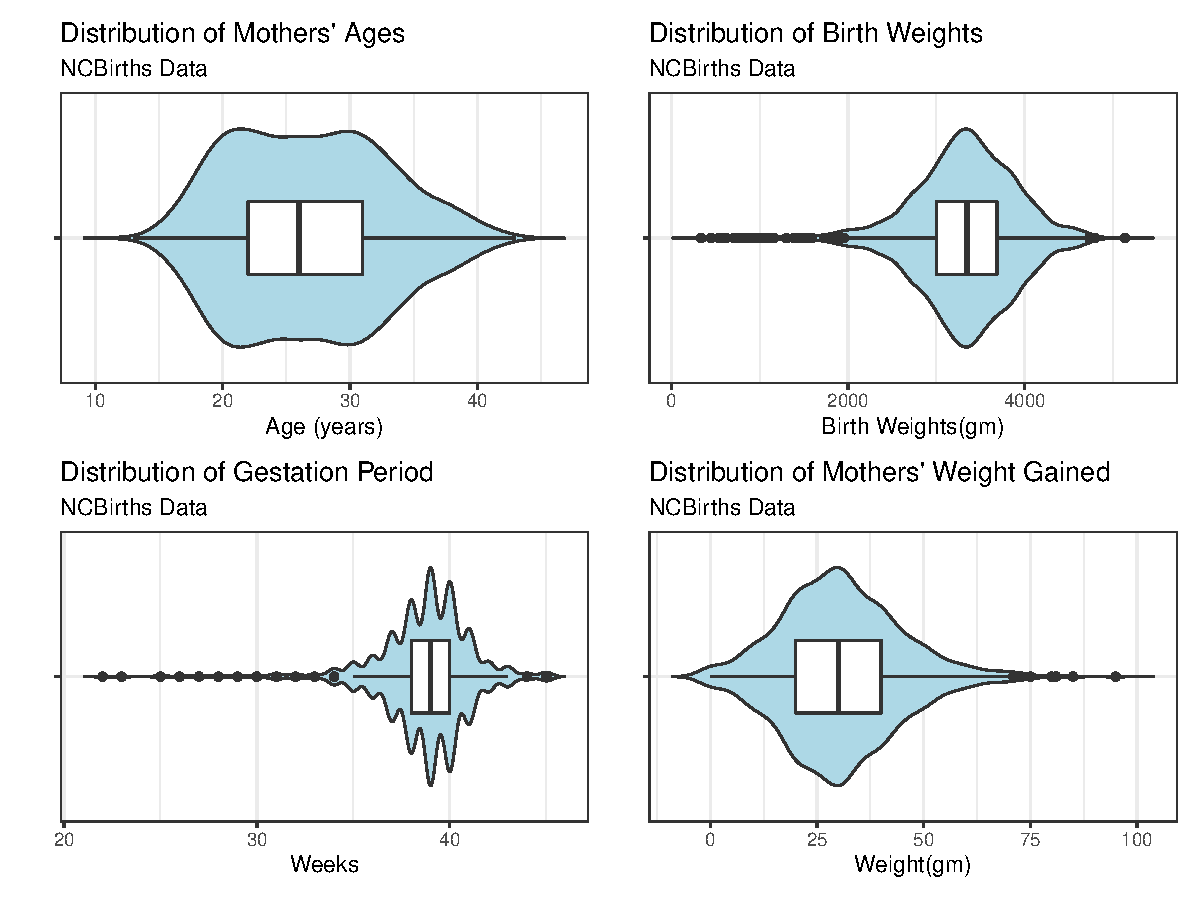
\includegraphics[width=\maxwidth]{figure/unnamed-chunk-3-1} 
\end{knitrout}
\caption{Violin plots of each variable.}
\label{ViolinSummary}
\end{figure}

the shape of the distribution of each variable
any unusual looking observations

From \ref{ViolinSummary} We can see that there is variability in almost all of the quantitative variables and they all have and many odd observations.

We also wanted to visualize the distributions of these variables.

\begin{knitrout}
\definecolor{shadecolor}{rgb}{0.969, 0.969, 0.969}\color{fgcolor}\begin{kframe}
\begin{alltt}
\hlstd{histogram.BirthWeight}\hlkwb{<-} \hlkwd{ggplot}\hlstd{(births,} \hlkwd{aes}\hlstd{(}\hlkwc{x}\hlstd{=BirthWeightGm))}\hlopt{+}
  \hlkwd{geom_histogram}\hlstd{(}\hlkwc{fill} \hlstd{=} \hlstr{"lightblue"}\hlstd{,}
                 \hlkwc{color} \hlstd{=} \hlstr{"black"}\hlstd{,}
                 \hlkwc{bins} \hlstd{=} \hlnum{5}\hlstd{)} \hlopt{+}
  \hlkwd{theme_bw}\hlstd{()} \hlopt{+}
  \hlkwd{xlab}\hlstd{(}\hlstr{"Birth Weights"}\hlstd{)}\hlopt{+}
  \hlkwd{ylab}\hlstd{(}\hlstr{"Count of Weight(gm)"}\hlstd{)}\hlopt{+}
  \hlkwd{ggtitle}\hlstd{(}\hlstr{"Frequencies of Birth Weights"}\hlstd{)}


\hlstd{histogram.Gestation}\hlkwb{<-} \hlkwd{ggplot}\hlstd{(births,} \hlkwd{aes}\hlstd{(}\hlkwc{x}\hlstd{=Weeks))}\hlopt{+}
  \hlkwd{geom_histogram}\hlstd{(}\hlkwc{fill} \hlstd{=} \hlstr{"lightblue"}\hlstd{,}
                 \hlkwc{color} \hlstd{=} \hlstr{"black"}\hlstd{,}
                 \hlkwc{bins} \hlstd{=} \hlnum{5}\hlstd{)} \hlopt{+}
  \hlkwd{theme_bw}\hlstd{()} \hlopt{+}
  \hlkwd{xlab}\hlstd{(}\hlstr{"Gestation Period"}\hlstd{)}\hlopt{+}
  \hlkwd{ylab}\hlstd{(}\hlstr{"Count of Weeks"}\hlstd{)}\hlopt{+}
  \hlkwd{ggtitle}\hlstd{(}\hlstr{"Frequencies of Gestation Periods"}\hlstd{)}

\hlstd{histogram.MomAge} \hlkwb{<-} \hlkwd{ggplot}\hlstd{(births,} \hlkwd{aes}\hlstd{(}\hlkwc{x}\hlstd{=MomAge))}\hlopt{+}
  \hlkwd{geom_histogram}\hlstd{(}\hlkwc{fill} \hlstd{=} \hlstr{"lightblue"}\hlstd{,}
                 \hlkwc{color} \hlstd{=} \hlstr{"black"}\hlstd{,}
                 \hlkwc{bins} \hlstd{=} \hlnum{5}\hlstd{)} \hlopt{+}
  \hlkwd{theme_bw}\hlstd{()} \hlopt{+}
  \hlkwd{xlab}\hlstd{(}\hlstr{"Ages of Mothers(years)"}\hlstd{)}\hlopt{+}
  \hlkwd{ylab}\hlstd{(}\hlstr{"Count of Ages"}\hlstd{)}\hlopt{+}
  \hlkwd{ggtitle}\hlstd{(}\hlstr{"Frequencies of Ages"}\hlstd{)}

\hlstd{histogram.BirthWeight} \hlopt{+} \hlstd{histogram.Gestation} \hlopt{+} \hlstd{histogram.MomAge}
\end{alltt}
\end{kframe}
\end{knitrout}

\begin{figure}[H]
\centering
\begin{knitrout}
\definecolor{shadecolor}{rgb}{0.969, 0.969, 0.969}\color{fgcolor}
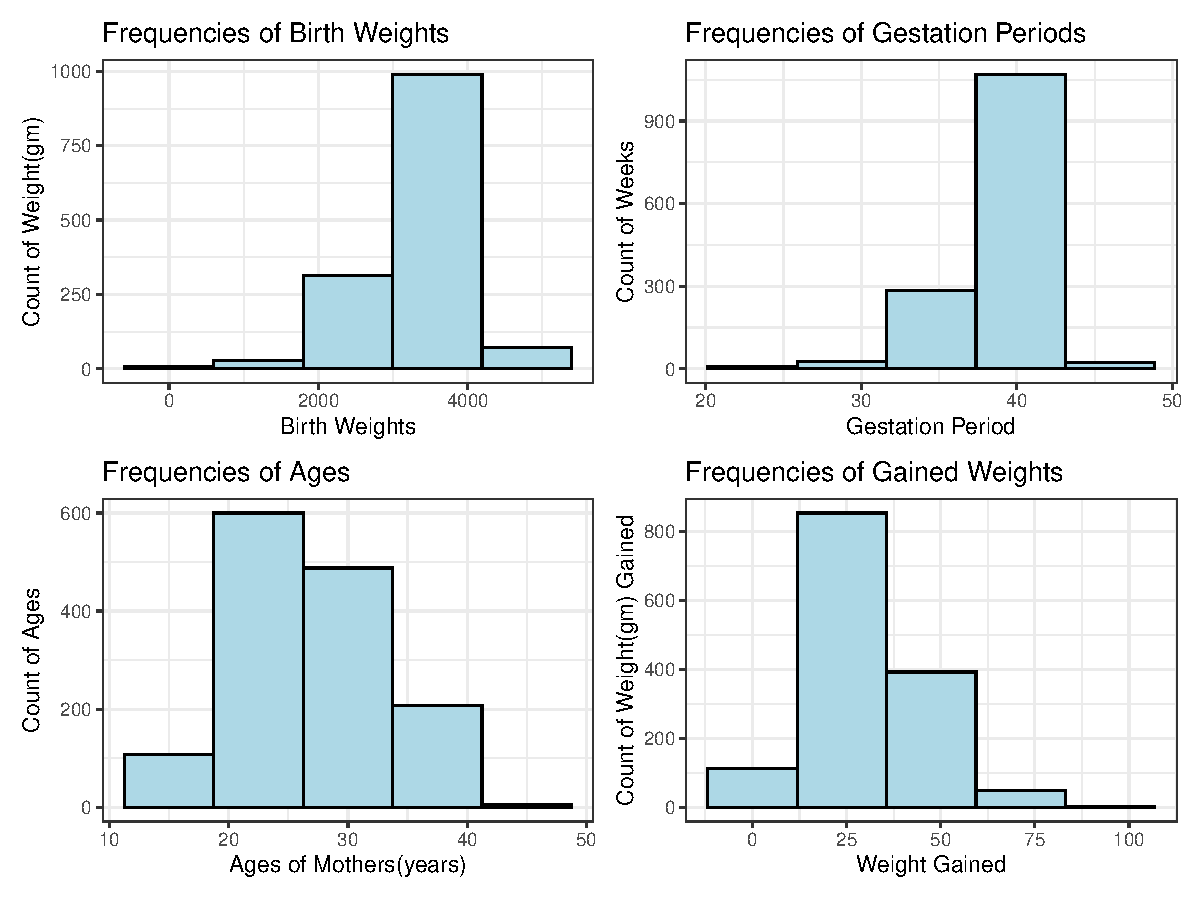
\includegraphics[width=\maxwidth]{figure/unnamed-chunk-4-1} 
\end{knitrout}
\caption{Grid of histograms for the quantitative variables.}
\label{HistogramSummary}
\end{figure}

\ref{HistogramSummary} shows that the quantitative variables do not follow normal distributions and are all skewed. 

We expected the distribution for weights and weeks to be similar in shape because typically babies that are born prematurely have low birth weights. We did find it interesting though, that the distributions showed more preemies that we initially expected. 

We weren't sure if the preemie weights in the data set were outlier instances that were heavily skewing the distribution, or if there were just more preemies that we expected. To further investigate this, we created a bootstrap confidence interval to see whether a baby born with a median weight falls within the interval. 

\begin{knitrout}
\definecolor{shadecolor}{rgb}{0.969, 0.969, 0.969}\color{fgcolor}\begin{kframe}
\begin{alltt}
\hlcom{## Bootstrapping for median weights }
\hlkwd{median}\hlstd{(births}\hlopt{$}\hlstd{BirthWeightGm)}
\end{alltt}
\begin{verbatim}
## [1] 3345.3
\end{verbatim}
\begin{alltt}
\hlkwd{set.seed}\hlstd{(}\hlnum{23}\hlstd{)}
\hlstd{alpha} \hlkwb{<-} \hlnum{0.05}
\hlstd{n} \hlkwb{<-} \hlkwd{nrow}\hlstd{(births)}
\hlstd{R} \hlkwb{<-} \hlnum{10000}
\hlstd{boot.stats} \hlkwb{<-} \hlkwd{rep}\hlstd{(}\hlnum{NA}\hlstd{, R)}
\hlkwa{for} \hlstd{(i} \hlkwa{in} \hlnum{1}\hlopt{:}\hlstd{R)\{}
  \hlstd{boot.data} \hlkwb{<-} \hlkwd{sample}\hlstd{(}\hlkwc{x} \hlstd{= births}\hlopt{$}\hlstd{BirthWeightGm,} \hlkwc{size} \hlstd{= n,} \hlkwc{replace} \hlstd{=} \hlnum{TRUE}\hlstd{)}
  \hlstd{boot.stats[i]} \hlkwb{<-} \hlkwd{median}\hlstd{(boot.data)}
\hlstd{\}}

\hlkwd{quantile}\hlstd{(boot.stats,} \hlkwc{probs} \hlstd{=} \hlkwd{c}\hlstd{(alpha}\hlopt{/}\hlnum{2}\hlstd{,} \hlnum{1} \hlopt{-} \hlstd{alpha}\hlopt{/}\hlnum{2}\hlstd{))}
\end{alltt}
\begin{verbatim}
##    2.5%   97.5% 
## 3316.95 3373.65
\end{verbatim}
\begin{alltt}
\hlstd{samp.boot.med} \hlkwb{<-} \hlkwa{function}\hlstd{(}\hlkwc{data}\hlstd{,} \hlkwc{indicies}\hlstd{)\{}
  \hlkwd{median}\hlstd{(data[indicies])}
\hlstd{\}}

\hlstd{boot.medians} \hlkwb{<-} \hlkwd{boot}\hlstd{(}\hlkwc{data} \hlstd{= births}\hlopt{$}\hlstd{BirthWeightGm,} \hlkwc{statistic} \hlstd{= samp.boot.med,} \hlkwc{R} \hlstd{=} \hlnum{10000}\hlstd{)}
\hlkwd{boot.ci}\hlstd{(boot.medians,} \hlkwc{conf} \hlstd{=} \hlnum{0.95}\hlstd{)}
\end{alltt}


{\ttfamily\noindent\color{warningcolor}{\#\# Warning in boot.ci(boot.medians, conf = 0.95): bootstrap variances needed for studentized intervals}}\begin{verbatim}
## BOOTSTRAP CONFIDENCE INTERVAL CALCULATIONS
## Based on 10000 bootstrap replicates
## 
## CALL : 
## boot.ci(boot.out = boot.medians, conf = 0.95)
## 
## Intervals : 
## Level      Normal              Basic         
## 95%   (3314, 3381 )   (3317, 3374 )  
## 
## Level     Percentile            BCa          
## 95%   (3317, 3374 )   (3289, 3345 )  
## Calculations and Intervals on Original Scale
## Some BCa intervals may be unstable
\end{verbatim}
\end{kframe}
\end{knitrout}

The median birth weight of our dataset was 3,345.3 grams. Our 95\% percentile confidence interval was 3316.95 g. to 3373.65 g. This range contained our median birth weight of 3,345.3 grams, but more than that, our confidence interval was extremely close to the reported statistics from the World Health Organization of median birth weight of 3.3 kg (The WHO did not include any additional significant figures, so we assume that this could range from values anywhere to 3.25 kg to 3.35 kg.). This seems to lend support to our decision to assume that the collected data was representative of the population, despite the lack of specific knowledge of the collection techniques. Further, it indicates to us that we have a reasonable sample even with its non-normal distribution, that was caused by its skew from data primarily relating to babies born prematurely. 

\item\textbf{Numerically summarize the variables in your dataset.}
\begin{knitrout}
\definecolor{shadecolor}{rgb}{0.969, 0.969, 0.969}\color{fgcolor}\begin{kframe}
\begin{alltt}
\hlcom{#add in weeks }
\hlstd{(sumstats} \hlkwb{<-} \hlstd{births} \hlopt \hlkwd{summarize}\hlstd{(}\hlkwc{meanW}\hlstd{=}\hlkwd{mean}\hlstd{(BirthWeightGm),}
                                 \hlkwc{medianW} \hlstd{=} \hlkwd{median}\hlstd{(BirthWeightGm),}
                                  \hlkwc{varianceW}\hlstd{=}\hlkwd{var}\hlstd{(BirthWeightGm),}
                                 \hlkwc{meanA}\hlstd{=}\hlkwd{mean}\hlstd{(MomAge),}
                                 \hlkwc{medianA}\hlstd{=}\hlkwd{median}\hlstd{(MomAge),}
                                 \hlkwc{varianceA} \hlstd{=} \hlkwd{var}\hlstd{(MomAge),}
                                 \hlkwc{meanWeeks} \hlstd{=} \hlkwd{mean}\hlstd{(Weeks),}
                                 \hlkwc{medianWeeks} \hlstd{=} \hlkwd{median}\hlstd{(Weeks),}
                                 \hlkwc{varianceWeeks} \hlstd{=} \hlkwd{var}\hlstd{(Weeks)))}
\end{alltt}
\begin{verbatim}
## # A tibble: 1 x 9
##   meanW medianW varianceW meanA medianA varianceA meanWeeks medianWeeks varian~1
##   <dbl>   <dbl>     <dbl> <dbl>   <dbl>     <dbl>     <dbl>       <dbl>    <dbl>
## 1 3301.   3345.   393454.  26.8      26      37.1      38.6          39     7.04
## # ... with abbreviated variable name 1: varianceWeeks
\end{verbatim}
\end{kframe}
\end{knitrout}

Tableu visual

\item\textbf{Create a scatterplot matrix and table of correlations.}
\begin{knitrout}
\definecolor{shadecolor}{rgb}{0.969, 0.969, 0.969}\color{fgcolor}\begin{kframe}
\begin{alltt}
\hlkwd{library}\hlstd{(GGally)}
\hlcom{#ADD IN CORRECT VARIABLE NAMES}
\hlstd{correlationsmatrix} \hlkwb{<-} \hlkwd{ggpairs}\hlstd{(births,} \hlkwc{columns} \hlstd{=} \hlkwd{c}\hlstd{())}

\hlstd{correlationsmatrix}
\end{alltt}
\end{kframe}
\end{knitrout}

\begin{figure}[H]
\centering
\begin{knitrout}
\definecolor{shadecolor}{rgb}{0.969, 0.969, 0.969}\color{fgcolor}\begin{kframe}


{\ttfamily\noindent\bfseries\color{errorcolor}{\#\# Error in data.frame(plotType = plotType, xVar = xVar, yVar = yVar, posX = posX, : arguments imply differing number of rows: 0, 1}}

{\ttfamily\noindent\bfseries\color{errorcolor}{\#\# Error in eval(expr, envir, enclos): object 'correlationsmatrix' not found}}\end{kframe}
\end{knitrout}
\caption{Matrix of ScatterPlots and Correlations for the variables.}
\label{CorrelationSummary}
\end{figure}

\item\textbf{Other interesting plots.}

Plot significant correlations 
- weeks and birth weight

\item\textbf{Comment on...}
\begin{enumerate}[]
\item{the shape of the distribution of each variable}
\item{the relationship between the response and the quantitative predictors}
\item{any unusual looking observations}
\item{any other interesting takeaways}
\end{enumerate}
\end{enumerate}

\section{Part 4: First-Order Model and Model Selection.}

First we created some functions that...

\begin{knitrout}
\definecolor{shadecolor}{rgb}{0.969, 0.969, 0.969}\color{fgcolor}\begin{kframe}
\begin{alltt}
\hlcom{#create functions}
\hlcom{#Calculates the residuals departure from the theoretical quantiles, returning the mean abs() value of the actual minus theoretical quantiles }
\hlstd{quantDepart} \hlkwb{<-} \hlkwa{function}\hlstd{(}\hlkwc{model}\hlstd{) \{}
  \hlstd{residuals} \hlkwb{<-} \hlkwd{sort}\hlstd{(}\hlkwd{scale}\hlstd{(model}\hlopt{$}\hlstd{residuals,} \hlkwc{scale}\hlstd{=T))}
  \hlstd{i} \hlkwb{<-} \hlnum{1}\hlopt{:}\hlkwd{length}\hlstd{(residuals)}
  \hlstd{fi} \hlkwb{<-} \hlstd{(i} \hlopt{-} \hlnum{0.5}\hlstd{)} \hlopt{/} \hlkwd{length}\hlstd{(residuals)}
  \hlstd{x.norm} \hlkwb{<-} \hlkwd{qnorm}\hlstd{(fi)}

  \hlkwd{mean}\hlstd{(}\hlkwd{abs}\hlstd{(residuals} \hlopt{-} \hlstd{x.norm))}
\hlstd{\}}

\hlcom{#Displays a variety of summary stats and graphics of the model tailored based off of the specific options attributes set to True}
\hlstd{modelSummary} \hlkwb{<-} \hlkwa{function}\hlstd{(}\hlkwc{model}\hlstd{,} \hlkwc{coef}\hlstd{=T,} \hlkwc{stat}\hlstd{=T,} \hlkwc{plot}\hlstd{=T)\{}
  \hlkwa{if}\hlstd{(coef) \{}
    \hlkwd{print}\hlstd{(}\hlkwd{round}\hlstd{(}\hlkwd{summary}\hlstd{(model)}\hlopt{$}\hlstd{coefficients,}\hlnum{10}\hlstd{))}
  \hlstd{\}}
  \hlkwa{if}\hlstd{(stat) \{}
    \hlkwd{print}\hlstd{(}\hlkwd{paste}\hlstd{(}\hlstr{"R-squared:"}\hlstd{,} \hlkwd{summary}\hlstd{(model)}\hlopt{$}\hlstd{r.squared))}
    \hlkwd{print}\hlstd{(}\hlkwd{paste}\hlstd{(}\hlstr{"Adjusted R-Squared:"}\hlstd{,} \hlkwd{summary}\hlstd{(model)}\hlopt{$}\hlstd{adj.r.squared))}
    \hlkwd{print}\hlstd{(}\hlkwd{paste}\hlstd{(}\hlstr{"Sigma:"}\hlstd{,} \hlkwd{summary}\hlstd{(model)}\hlopt{$}\hlstd{sigma))}
    \hlkwd{print}\hlstd{(}\hlkwd{paste}\hlstd{(}\hlstr{"AIC:"}\hlstd{,} \hlkwd{AIC}\hlstd{(model)))}
    \hlkwd{print}\hlstd{(}\hlkwd{paste}\hlstd{(}\hlstr{"BIC:"}\hlstd{,} \hlkwd{BIC}\hlstd{(model)))}
    \hlkwd{print}\hlstd{(}\hlkwd{paste}\hlstd{(}\hlstr{"Quantile Departure:"}\hlstd{,} \hlkwd{quantDepart}\hlstd{(model)))}
  \hlstd{\}}
  \hlkwa{if}\hlstd{(plot) \{}
    \hlkwd{plotResiduals}\hlstd{(model)}
  \hlstd{\}}
\hlstd{\}}

\hlcom{#Calculates the  R squared of predicted vs actual values }
\hlstd{r_squared} \hlkwb{<-} \hlkwa{function}\hlstd{(}\hlkwc{actual}\hlstd{,} \hlkwc{predicted}\hlstd{) \{}
  \hlkwd{cor}\hlstd{(actual, predicted)}\hlopt{^}\hlnum{2}
\hlstd{\}}

\hlcom{#If provided with a model and a number of subsets of data, this will generate summary statistics for those subsets }
\hlstd{predictForSubsets} \hlkwb{<-} \hlkwa{function}\hlstd{(}\hlkwc{model}\hlstd{,} \hlkwc{class.attr}\hlstd{,} \hlkwc{...}\hlstd{) \{}
  \hlstd{x} \hlkwb{<-} \hlkwd{list}\hlstd{(...)}
  \hlstd{i} \hlkwb{<-} \hlnum{1}
  \hlstd{predPlots} \hlkwb{=} \hlkwd{list}\hlstd{()}
  \hlstd{residPlots} \hlkwb{=} \hlkwd{list}\hlstd{()}
  \hlkwa{for} \hlstd{(v} \hlkwa{in} \hlstd{x) \{}
    \hlstd{v}\hlopt{$}\hlstd{predict} \hlkwb{<-} \hlkwd{predict}\hlstd{(model, v)}
    \hlstd{v}\hlopt{$}\hlstd{resid} \hlkwb{<-} \hlstd{v[[class.attr]]} \hlopt{-} \hlstd{v}\hlopt{$}\hlstd{predict}


    \hlkwd{print}\hlstd{(}\hlkwd{paste}\hlstd{(}\hlstr{"Subset"}\hlstd{, i,} \hlstr{"R-Squared:"}\hlstd{,} \hlkwd{r_squared}\hlstd{(v}\hlopt{$}\hlstd{predict, v[[class.attr]])))}
    \hlkwd{print}\hlstd{(}\hlkwd{paste}\hlstd{(}\hlstr{"Subset"}\hlstd{, i,} \hlstr{"Mean Abs. Error:"}\hlstd{,} \hlkwd{mean}\hlstd{(}\hlkwd{abs}\hlstd{(v}\hlopt{$}\hlstd{resid))))}

    \hlkwd{ggplot}\hlstd{(}\hlkwc{data}\hlstd{=v,} \hlkwd{aes}\hlstd{(}\hlkwc{x}\hlstd{=predict,} \hlkwc{y}\hlstd{=resid))} \hlopt{+}
      \hlkwd{geom_point}\hlstd{(}\hlkwc{size}\hlstd{=}\hlnum{1}\hlstd{,}
                 \hlkwc{shape}\hlstd{=}\hlnum{16}\hlstd{)}\hlopt{+}
      \hlkwd{theme_bw}\hlstd{()}\hlopt{+}
      \hlkwd{xlab}\hlstd{(}\hlstr{"Predicted"}\hlstd{)}\hlopt{+}
      \hlkwd{ylab}\hlstd{(}\hlstr{"Residuals"}\hlstd{)}\hlopt{+}
      \hlkwd{ggtitle}\hlstd{(}\hlstr{"Predicted versus Residuals"}\hlstd{)} \hlkwb{->} \hlstd{residuals}
    \hlkwd{ggplot}\hlstd{(}\hlkwc{data}\hlstd{=v,} \hlkwd{aes}\hlstd{(}\hlkwc{x}\hlstd{=predict,} \hlkwc{y}\hlstd{=}\hlkwd{get}\hlstd{(class.attr)))} \hlopt{+}
      \hlkwd{geom_point}\hlstd{(}\hlkwc{size}\hlstd{=}\hlnum{1}\hlstd{,}
                 \hlkwc{shape}\hlstd{=}\hlnum{16}\hlstd{)}\hlopt{+}
      \hlkwd{theme_bw}\hlstd{()}\hlopt{+}
      \hlkwd{xlab}\hlstd{(}\hlstr{"Predicted"}\hlstd{)}\hlopt{+}
      \hlkwd{ylab}\hlstd{(}\hlstr{"Actual"}\hlstd{)}\hlopt{+}
      \hlkwd{ggtitle}\hlstd{(}\hlstr{"Predicted versus Actual"}\hlstd{)} \hlkwb{->} \hlstd{predictions}
    \hlkwd{print}\hlstd{(predictions} \hlopt{+} \hlstd{residuals)}
    \hlstd{i} \hlkwb{<-} \hlstd{i} \hlopt{+} \hlnum{1}
  \hlstd{\}}
\hlstd{\}}
\end{alltt}
\end{kframe}
\end{knitrout}

\subsection{First Order Model}

First, we fit a first-order linear model with all of our predictors. The estimated linear regression equation is \\

\begin{align*} \hat{y} &= -964.29 + -704.71\cdot \text{I}(\text{Plural} = 2) + -932.13\cdot \text{I}(\text{Plural} = 3) + 93.90\cdot \text{I}(\text{Sex} = \text{Male}) \\ &\quad + 10.88\cdot \text{MomAge} + 97.81\cdot \text{Weeks} -76.88\cdot \text{I}(\text{RaceMom} = \text{Black}) + 81.31\cdot \text{I}(\text{RaceMom} = \text{Chinese}) \\ &\quad -860.40\cdot \text{I}(\text{RaceMom} = \text{Filipino}) + 29.04\cdot \text{I}(\text{RaceMom} = \text{Japanese}) -58.43\cdot \text{I}(\text{RaceMom} = \text{Other\ Asian/PI}) \\ &\quad + 30.78\cdot \text{I}(\text{RaceMom} = \text{White}) -48.07\cdot \text{I}(\text{Marital} = \text{Unmarried}) + 7.87\cdot \text{Gained} \\ &\quad -203.49\cdot \text{I}(\text{Smoke} = \text{Yes}) -217.62\cdot \text{I}(\text{Premie} = \text{Yes}) \end{align*}
  
  
\begin{knitrout}
\definecolor{shadecolor}{rgb}{0.969, 0.969, 0.969}\color{fgcolor}\begin{kframe}
\begin{alltt}
\hlcom{#first model = model.1}
\hlkwd{lm}\hlstd{(BirthWeightGm} \hlopt{~} \hlstd{Plural} \hlopt{+} \hlstd{Sex} \hlopt{+} \hlstd{MomAge} \hlopt{+} \hlstd{Weeks} \hlopt{+} \hlstd{RaceMom} \hlopt{+}
     \hlstd{Marital} \hlopt{+} \hlstd{Gained} \hlopt{+} \hlstd{Smoke} \hlopt{+} \hlstd{Premie, births)} \hlkwb{->} \hlstd{model.1}

\hlkwd{modelSummary}\hlstd{(model.1,} \hlkwc{coef} \hlstd{=} \hlnum{TRUE}\hlstd{)}
\end{alltt}
\begin{verbatim}
##                           Estimate  Std. Error    t value     Pr(>|t|)
## (Intercept)             -964.28919 294.9607224 -3.2692122 0.0011048007
## Plural2                 -704.70670  76.5727750 -9.2030973 0.0000000000
## Plural3                 -932.12784 237.3884857 -3.9265925 0.0000903705
## SexMale                   93.89649  24.8249532  3.7823432 0.0001619382
## MomAge                    10.88077   2.3232147  4.6834980 0.0000030955
## Weeks                     97.81144   6.8023799 14.3790033 0.0000000000
## RaceMomBlack             -76.87702 102.7336877 -0.7483137 0.4543973043
## RaceMomChinese            81.30745 344.1690322  0.2362428 0.8132790072
## RaceMomFilipino         -860.40322 476.1359772 -1.8070536 0.0709696081
## RaceMomJapanese           29.03632 106.7611068  0.2719747 0.7856817781
## RaceMomOther Asian / PI  -58.43107 140.9347082 -0.4145967 0.6785009952
## RaceMomWhite              30.78400 101.2713293  0.3039755 0.7611919583
## MaritalUnmarried         -48.07301  32.1293957 -1.4962315 0.1348198655
## Gained                     7.86655   0.9098714  8.6457814 0.0000000000
## SmokeYes                -203.48734  36.5920140 -5.5609767 0.0000000321
## PremieYes               -217.62136  53.3527133 -4.0789183 0.0000478089
## [1] "R-squared: 0.45706523101896"
## [1] "Adjusted R-Squared: 0.451218840828927"
## [1] "Sigma: 464.671921644458"
## [1] "AIC: 21322.7497301962"
## [1] "BIC: 21412.0105338985"
## [1] "Quantile Departure: 0.0472456539674342"
\end{verbatim}
\end{kframe}
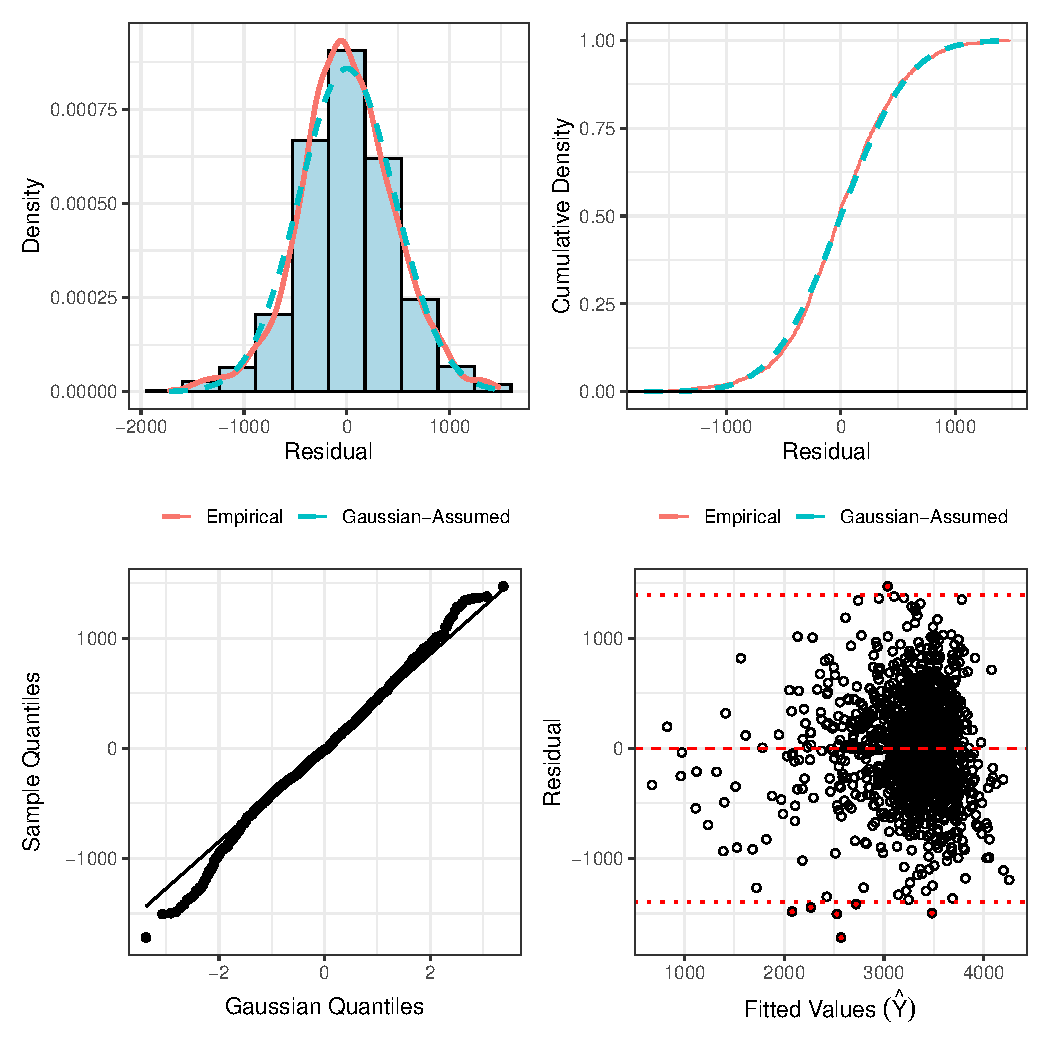
\includegraphics[width=\maxwidth]{figure/unnamed-chunk-9-1} 
\begin{kframe}\begin{alltt}
\hlkwd{xtable}\hlstd{(model.1,} \hlkwc{caption}\hlstd{=}\hlstr{"Predictor Statistics and Significance"}\hlstd{,} \hlkwc{label}\hlstd{=}\hlstr{"First.Order.Table"}\hlstd{)}
\end{alltt}
\begin{verbatim}
## % latex table generated in R 4.2.1 by xtable 1.8-4 package
## % Wed Dec  7 17:31:29 2022
## \begin{table}[ht]
## \centering
## \begin{tabular}{rrrrr}
##   \hline
##  & Estimate & Std. Error & t value & Pr($>$$|$t$|$) \\ 
##   \hline
## (Intercept) & -964.2892 & 294.9607 & -3.27 & 0.0011 \\ 
##   Plural2 & -704.7067 & 76.5728 & -9.20 & 0.0000 \\ 
##   Plural3 & -932.1278 & 237.3885 & -3.93 & 0.0001 \\ 
##   SexMale & 93.8965 & 24.8250 & 3.78 & 0.0002 \\ 
##   MomAge & 10.8808 & 2.3232 & 4.68 & 0.0000 \\ 
##   Weeks & 97.8114 & 6.8024 & 14.38 & 0.0000 \\ 
##   RaceMomBlack & -76.8770 & 102.7337 & -0.75 & 0.4544 \\ 
##   RaceMomChinese & 81.3075 & 344.1690 & 0.24 & 0.8133 \\ 
##   RaceMomFilipino & -860.4032 & 476.1360 & -1.81 & 0.0710 \\ 
##   RaceMomJapanese & 29.0363 & 106.7611 & 0.27 & 0.7857 \\ 
##   RaceMomOther Asian / PI & -58.4311 & 140.9347 & -0.41 & 0.6785 \\ 
##   RaceMomWhite & 30.7840 & 101.2713 & 0.30 & 0.7612 \\ 
##   MaritalUnmarried & -48.0730 & 32.1294 & -1.50 & 0.1348 \\ 
##   Gained & 7.8665 & 0.9099 & 8.65 & 0.0000 \\ 
##   SmokeYes & -203.4873 & 36.5920 & -5.56 & 0.0000 \\ 
##   PremieYes & -217.6214 & 53.3527 & -4.08 & 0.0000 \\ 
##    \hline
## \end{tabular}
## \caption{Predictor Statistics and Significance} 
## \label{First.Order.Table}
## \end{table}
\end{verbatim}
\end{kframe}
\end{knitrout}

\begin{table}[ht]
\centering
\begin{tabular}{lrrrrr}
  \hline
R-Squared & Adjusted R-Squared & RSE & AIC & BIC\\ 
  \hline
   0.4570 & 0.4512 & 464.6719 & 21322.7497 & 21412.0105 \\ 
   \hline
\end{tabular}
\caption{Summary of first order regression model R-squared, Adj R-squared, RSE, AIC, and BIC.}
\label{first.order.summary}
\end{table}

As Table \ref{First.Order.Table} indicates, Plural2 (Twins), Plural3 (Triplets), Sex = Male, MomAge, Weeks, RaceMom = Filipino, Gained, Smoke = Yes, and Premie = Yes are all significant predictors. Table \ref{first.order.summary} demonstrates that the R-squared is is fairly high, meaning the model is quite predictive; however, AIC and BIC values are also extremely high, meaning that the number of predictor variables is not predictive enough to justify the variety of parameters we are using.

\begin{knitrout}
\definecolor{shadecolor}{rgb}{0.969, 0.969, 0.969}\color{fgcolor}\begin{kframe}
\begin{alltt}
\hlkwd{plotResiduals}\hlstd{(model.1)}
\end{alltt}
\end{kframe}
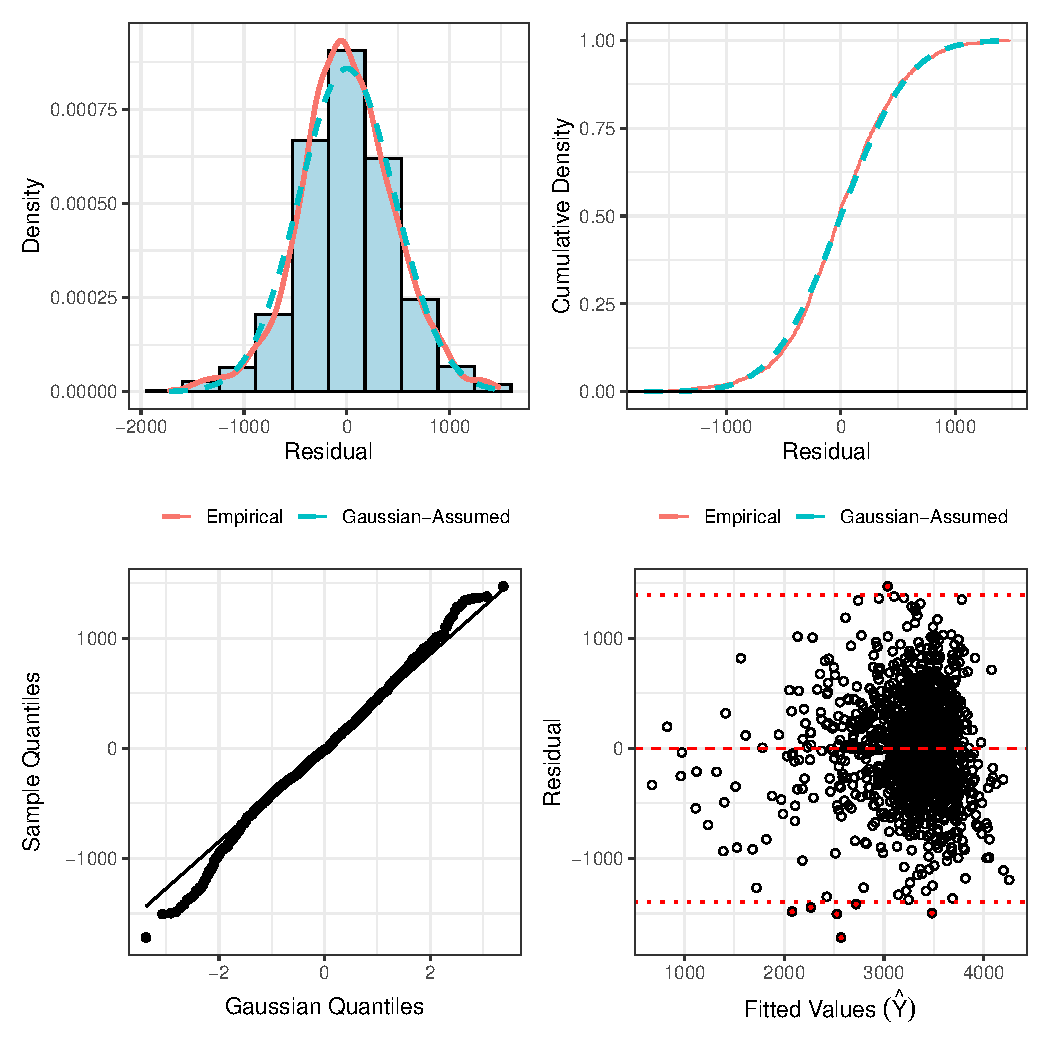
\includegraphics[width=\maxwidth]{figure/unnamed-chunk-10-1} 
\end{knitrout}

Before eliminating the non-significant variables from our model we wanted to test transformations of BirthWeight, to improve residual distribution. The model statistics for each transformation are listed in the table below. 

\begin{table}[ht]
\centering
\begin{tabular}{lrrrrrr}
  \hline
  Transformation & R-Squared & Adjusted R-Squared & RSE & AIC & BIC\\ 
  \hline
   First-order Model & 0.4570 & 0.4512 & 464.6719 & 21322.7497 & 21412.0105 \\ 
   Log of Weight & 0.5243 & 0.5192 & 0.1756 & -885.2705 & -796.0097\\ 
   Square Root of Weight & 0.4994 & 0.4940 & 4.3160 & 8137.3786 & 8226.6394\\
   Weight Squared & 0.3699 & 0.3631 & 3044641.3454 & 46086.0996 & 46175.3604\\
   Log of Weight Squared & 0.5208 & 0.5156 & 2.6968 & 6812.1540 & 6901.4149\\
   Log of the Log of Weight & 0.5249 & 0.5198 & 0.0231 & -6597.7982 & -6508.5374\\
   Log of the Square Root of Weight & 0.5243 & 0.5192 & 0.3512 & 1068.0181 & 1157.2789\\
   Square Root of the Log of Weight & 0.5250 & 0.5199 & 0.0318 & -5699.0284 & -5609.7676\\
   Inverse of the Weight & 0.5250 & 0.5199 & 0.0318 & -5699.0284 & -5609.7676\\
   \hline
\end{tabular}
\caption{Summary of all adjusted first order regression model R-squared, Adj R-squared, RSE, AIC, and BIC.}
\end{table}

\begin{knitrout}
\definecolor{shadecolor}{rgb}{0.969, 0.969, 0.969}\color{fgcolor}\begin{kframe}
\begin{alltt}
\hlcom{# Log of Weight}
\hlkwd{lm}\hlstd{(WeightGmLog} \hlopt{~} \hlstd{Plural} \hlopt{+} \hlstd{Sex} \hlopt{+} \hlstd{MomAgeSC} \hlopt{+} \hlstd{WeeksSC} \hlopt{+} \hlstd{RaceMom} \hlopt{+}
     \hlstd{Marital} \hlopt{+} \hlstd{GainedSC} \hlopt{+} \hlstd{Smoke} \hlopt{+} \hlstd{Premie, births)} \hlkwb{->} \hlstd{model.log}

\hlcom{# Square Root of Weight}
\hlkwd{lm}\hlstd{(WeightGmSqrt} \hlopt{~} \hlstd{Plural} \hlopt{+} \hlstd{Sex} \hlopt{+} \hlstd{MomAgeSC} \hlopt{+} \hlstd{WeeksSC} \hlopt{+} \hlstd{RaceMom} \hlopt{+}
     \hlstd{Marital} \hlopt{+} \hlstd{GainedSC} \hlopt{+} \hlstd{Smoke} \hlopt{+} \hlstd{Premie, births)} \hlkwb{->} \hlstd{model.sqrt}

\hlcom{# Squared of Weight}
\hlkwd{lm}\hlstd{(WeightGmS} \hlopt{~} \hlstd{Plural} \hlopt{+} \hlstd{Sex} \hlopt{+} \hlstd{MomAgeSC} \hlopt{+} \hlstd{WeeksSC} \hlopt{+} \hlstd{RaceMom} \hlopt{+}
     \hlstd{Marital} \hlopt{+} \hlstd{GainedSC} \hlopt{+} \hlstd{Smoke} \hlopt{+} \hlstd{Premie, births)} \hlkwb{->} \hlstd{model.s}

\hlcom{# Square of the Log of Weight}
\hlkwd{lm}\hlstd{(WeightGmSLog} \hlopt{~} \hlstd{Plural} \hlopt{+} \hlstd{Sex} \hlopt{+} \hlstd{MomAgeSC} \hlopt{+} \hlstd{WeeksSC} \hlopt{+} \hlstd{RaceMom} \hlopt{+}
     \hlstd{Marital} \hlopt{+} \hlstd{GainedSC} \hlopt{+} \hlstd{Smoke} \hlopt{+} \hlstd{Premie, births)} \hlkwb{->} \hlstd{model.slog}

\hlcom{# Log of the Log of Weight}
\hlkwd{lm}\hlstd{(WeightGmLogLog} \hlopt{~} \hlstd{Plural} \hlopt{+} \hlstd{Sex} \hlopt{+} \hlstd{MomAgeSC} \hlopt{+} \hlstd{WeeksSC} \hlopt{+} \hlstd{RaceMom} \hlopt{+}
     \hlstd{Marital} \hlopt{+} \hlstd{GainedSC} \hlopt{+} \hlstd{Smoke} \hlopt{+} \hlstd{Premie, births)} \hlkwb{->} \hlstd{model.loglog}

\hlcom{# Log of the Square Root of Weight}
\hlkwd{lm}\hlstd{(WeightGmLogSqr} \hlopt{~} \hlstd{Plural} \hlopt{+} \hlstd{Sex} \hlopt{+} \hlstd{MomAgeSC} \hlopt{+} \hlstd{WeeksSC} \hlopt{+} \hlstd{RaceMom} \hlopt{+}
     \hlstd{Marital} \hlopt{+} \hlstd{GainedSC} \hlopt{+} \hlstd{Smoke} \hlopt{+} \hlstd{Premie, births)} \hlkwb{->} \hlstd{model.logsqr}

\hlcom{# Square Root of the Log of Weight}
\hlkwd{lm}\hlstd{(WeightGmSqrtLog} \hlopt{~} \hlstd{Plural} \hlopt{+} \hlstd{Sex} \hlopt{+} \hlstd{MomAgeSC} \hlopt{+} \hlstd{WeeksSC} \hlopt{+} \hlstd{RaceMom} \hlopt{+}
     \hlstd{Marital} \hlopt{+} \hlstd{GainedSC} \hlopt{+} \hlstd{Smoke} \hlopt{+} \hlstd{Premie, births)} \hlkwb{->} \hlstd{model.sqrtlog}

\hlcom{# Inverse of the Weight}
\hlkwd{lm}\hlstd{(WeightGmInverse} \hlopt{~} \hlstd{Plural} \hlopt{+} \hlstd{Sex} \hlopt{+} \hlstd{MomAgeSC} \hlopt{+} \hlstd{WeeksSC} \hlopt{+} \hlstd{RaceMom} \hlopt{+}
     \hlstd{Marital} \hlopt{+} \hlstd{GainedSC} \hlopt{+} \hlstd{Smoke} \hlopt{+} \hlstd{Premie, births)} \hlkwb{->} \hlstd{model.inverse}
\end{alltt}
\end{kframe}
\end{knitrout}

At this point, we have two potential "best models": the un-transformed weight, which
better satisfies the assumptions behind linear regression modeling, namely the equal
distribution of residuals. We also have the log weight model, which has higher r-squared values and lower sigma, AIC, and BIC values than most other models, meaning it is more accurate. This accuracy is, however, gained only at the expense of making residuals less equally distributed, and thus satisfies the assumptions necessary to do things like conduct statistical inference on parameters. Thus, we will be proceeding with two models, the assumptions model and the accuracy model, where one will seek to minimize departure from assumptions and the other will seek to maximize accuracy. Assumption models will use the scaled and centered gram weight as their target, while accuracy models will use the scaled and centered log of gram weight.

Below is our current First-Order Model with all appropriate transformations, and numeric attributes scaled and centered.

\begin{knitrout}
\definecolor{shadecolor}{rgb}{0.969, 0.969, 0.969}\color{fgcolor}\begin{kframe}
\begin{alltt}
\hlcom{#First-Order Model with All Appropriate Transformations, and Numeric Attributes Scaled & Centered}
\hlkwd{lm}\hlstd{(WeightGmSC} \hlopt{~} \hlstd{Plural} \hlopt{+} \hlstd{Sex} \hlopt{+} \hlstd{MomAgeSC} \hlopt{+} \hlstd{WeeksSC} \hlopt{+} \hlstd{RaceMom} \hlopt{+}
     \hlstd{Marital} \hlopt{+} \hlstd{GainedSC} \hlopt{+} \hlstd{Smoke} \hlopt{+} \hlstd{Premie, births)} \hlkwb{->} \hlstd{model.2.assu}

\hlkwd{modelSummary}\hlstd{(model.2.assu)}
\end{alltt}
\begin{verbatim}
##                            Estimate Std. Error    t value     Pr(>|t|)
## (Intercept)              0.07028229 0.16262733  0.4321678 0.6656863816
## Plural2                 -1.12347022 0.12207523 -9.2030973 0.0000000000
## Plural3                 -1.48603366 0.37845375 -3.9265925 0.0000903705
## SexMale                  0.14969336 0.03957688  3.7823432 0.0001619382
## MomAgeSC                 0.10576700 0.02258291  4.6834980 0.0000030955
## WeeksSC                  0.42088560 0.02927085 14.3790033 0.0000000000
## RaceMomBlack            -0.12256027 0.16378195 -0.7483137 0.4543973043
## RaceMomChinese           0.12962343 0.54868736  0.2362428 0.8132790072
## RaceMomFilipino         -1.37168754 0.75907408 -1.8070536 0.0709696081
## RaceMomJapanese          0.04629081 0.17020262  0.2719747 0.7856817781
## RaceMomOther Asian / PI -0.09315303 0.22468347 -0.4145967 0.6785009952
## RaceMomWhite             0.04907703 0.16145060  0.3039755 0.7611919583
## MaritalUnmarried        -0.07663983 0.05122190 -1.4962315 0.1348198655
## GainedSC                 0.17403975 0.02013002  8.6457814 0.0000000000
## SmokeYes                -0.32440725 0.05833638 -5.5609767 0.0000000321
## PremieYes               -0.34694024 0.08505692 -4.0789183 0.0000478089
## [1] "R-squared: 0.457065231018961"
## [1] "Adjusted R-Squared: 0.451218840828928"
## [1] "Sigma: 0.740797650624698"
## [1] "AIC: 3170.99900079143"
## [1] "BIC: 3260.25980449371"
## [1] "Quantile Departure: 0.0472456539674346"
\end{verbatim}
\end{kframe}
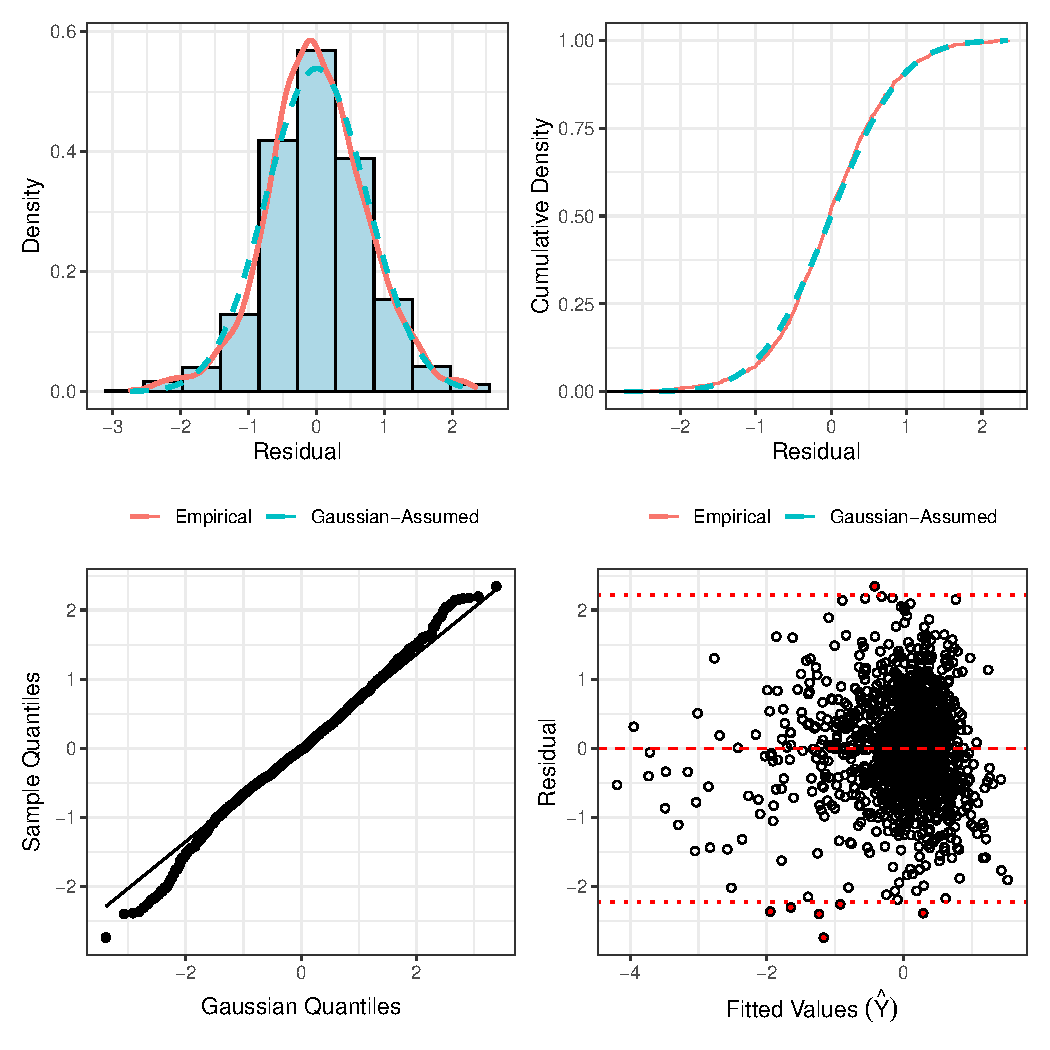
\includegraphics[width=\maxwidth]{figure/unnamed-chunk-12-1} 
\end{knitrout}

\begin{align*} 
\hat{y} &= 0.0703 -1.1235\cdot \text{Twin} -1.4860\cdot \text{Triplet} + 0.1497\cdot \text{I}(\text{Sex} = \text{Male}) \\ &\quad + 0.1058\cdot \text{MomAgeSC} + 0.4209\cdot \text{WeeksSC} \\ &\quad -0.1226\cdot \text{I}(\text{RaceMom} = \text{Black}) + 0.1296\cdot \text{I}(\text{RaceMom} = \text{Chinese}) \\ &\quad -1.3717\cdot \text{I}(\text{RaceMom} = \text{Filipino}) + 0.0463\cdot \text{I}(\text{RaceMom} = \text{Japanese}) \\ &\quad -0.0932\cdot \text{I}(\text{RaceMom} = \text{Other\ Asian/PI}) + 0.0491\cdot \text{I}(\text{RaceMom} = \text{White}) \\ &\quad -0.0766\cdot \text{I}(\text{Marital} = \text{Unmarried}) + 0.1740\cdot \text{GainedSC} \\ &\quad -0.3244\cdot \text{I}(\text{Smoke} = \text{Yes}) -0.3469\cdot \text{I}(\text{Premie} = \text{Yes}) 
\end{align*}

After obtaining our new model, we were curious as to how some of the predictors influenced the data set. Preemie means that the baby was born weeks before the predicted due date, and its commonly known that preemies have low birth weights. 

The code below tests the model on the data subset that only includes preemies, and the data subset that excludes preemies. We then ran the model on both and compared the results. 

\begin{knitrout}
\definecolor{shadecolor}{rgb}{0.969, 0.969, 0.969}\color{fgcolor}\begin{kframe}
\begin{alltt}
\hlkwd{predictForSubsets}\hlstd{(model.2.assu,} \hlstr{"WeightGmSC"}\hlstd{,}
                  \hlstd{births,}
                  \hlstd{births} \hlopt \hlkwd{filter}\hlstd{(Premie}\hlopt{==}\hlstr{"Yes"}\hlstd{),}
                  \hlstd{births} \hlopt \hlkwd{filter}\hlstd{(Premie}\hlopt{==}\hlstr{"No"}\hlstd{))}
\end{alltt}
\begin{verbatim}
## [1] "Subset 1 R-Squared: 0.457065231018961"
## [1] "Subset 1 Mean Abs. Error: 0.571443438631823"
\end{verbatim}
\end{kframe}
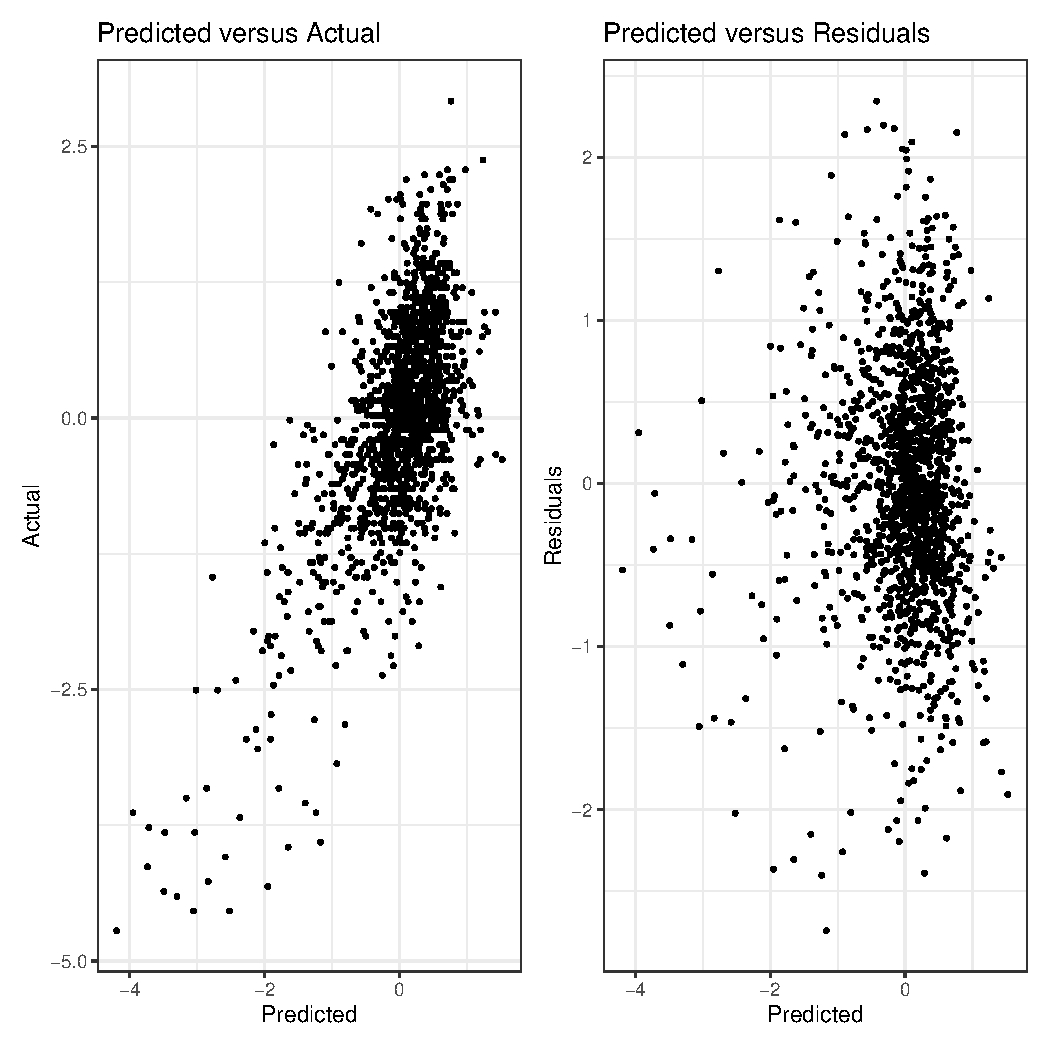
\includegraphics[width=\maxwidth]{figure/unnamed-chunk-13-1} 
\begin{kframe}\begin{verbatim}
## [1] "Subset 2 R-Squared: 0.551006218232442"
## [1] "Subset 2 Mean Abs. Error: 0.709020485309315"
\end{verbatim}
\end{kframe}
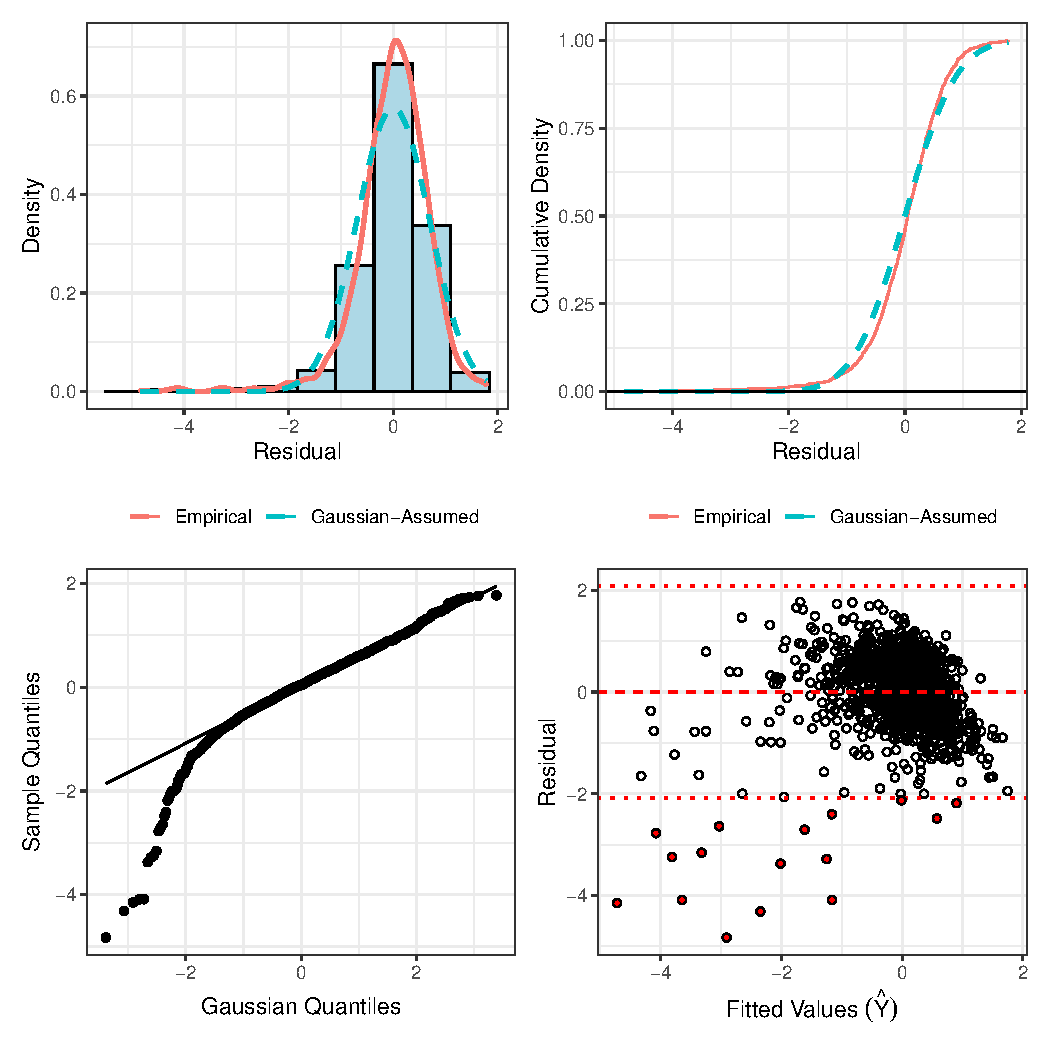
\includegraphics[width=\maxwidth]{figure/unnamed-chunk-13-2} 
\begin{kframe}\begin{verbatim}
## [1] "Subset 3 R-Squared: 0.175512160348786"
## [1] "Subset 3 Mean Abs. Error: 0.551165388592225"
\end{verbatim}
\end{kframe}
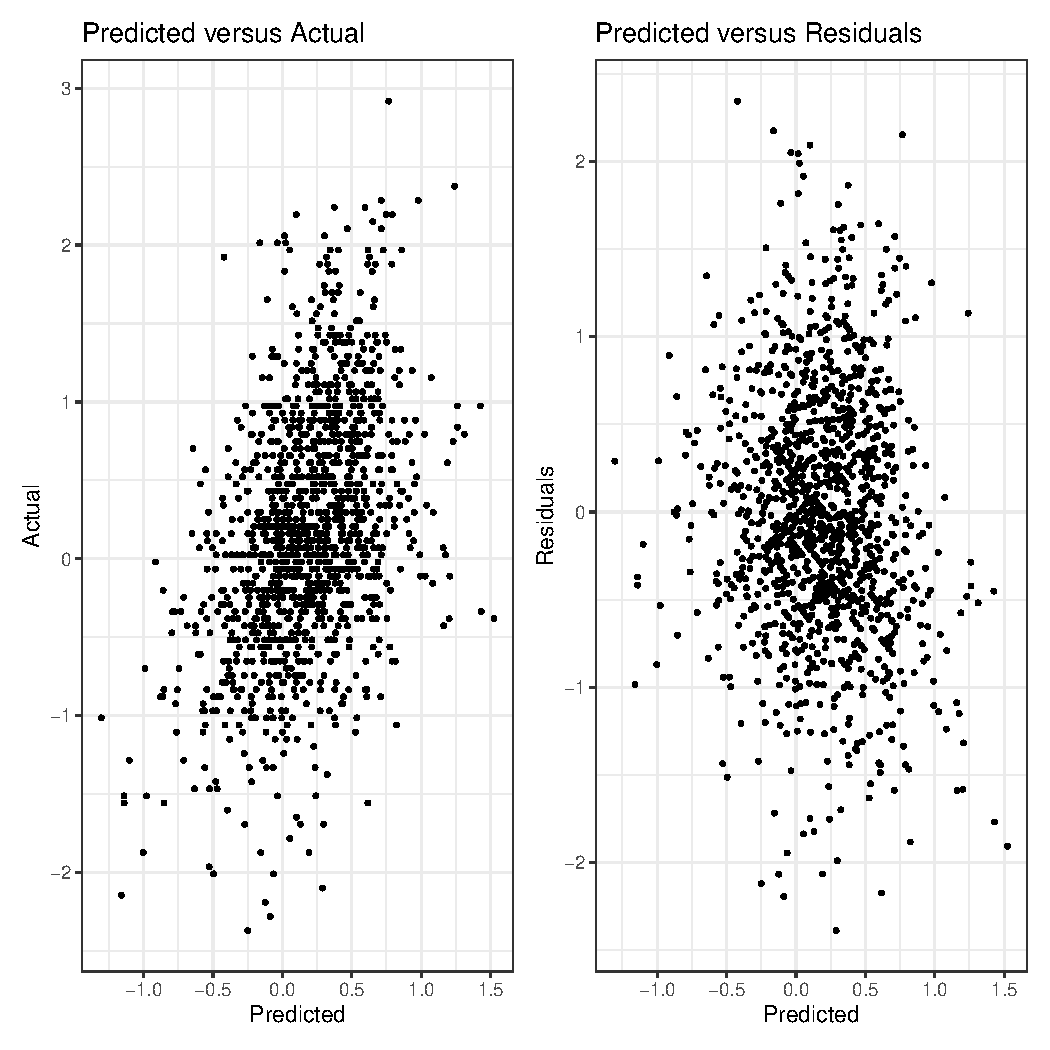
\includegraphics[width=\maxwidth]{figure/unnamed-chunk-13-3} 
\begin{kframe}\begin{alltt}
\hlkwd{lm}\hlstd{(WeightLogSC} \hlopt{~} \hlstd{Plural} \hlopt{+} \hlstd{Sex} \hlopt{+} \hlstd{MomAgeSC} \hlopt{+} \hlstd{WeeksSC} \hlopt{+} \hlstd{RaceMom} \hlopt{+}
     \hlstd{Marital} \hlopt{+} \hlstd{GainedSC} \hlopt{+} \hlstd{Smoke} \hlopt{+} \hlstd{Premie, births)} \hlkwb{->} \hlstd{model.2.accur}

\hlkwd{modelSummary}\hlstd{(model.2.accur)}
\end{alltt}
\begin{verbatim}
##                            Estimate Std. Error     t value     Pr(>|t|)
## (Intercept)              0.10329787 0.15222022  0.67860807 0.4974989472
## Plural2                 -1.01191972 0.11426320 -8.85604241 0.0000000000
## Plural3                 -1.55437979 0.35423513 -4.38798876 0.0000123026
## SexMale                  0.10769027 0.03704422  2.90707360 0.0037060130
## MomAgeSC                 0.10189593 0.02113775  4.82056744 0.0000015884
## WeeksSC                  0.55647332 0.02739770 20.31095005 0.0000000000
## RaceMomBlack            -0.15127673 0.15330096 -0.98679577 0.3239141352
## RaceMomChinese           0.14223435 0.51357488  0.27694959 0.7818599036
## RaceMomFilipino         -1.20670223 0.71049820 -1.69838886 0.0896577113
## RaceMomJapanese          0.01131033 0.15931074  0.07099541 0.9434115974
## RaceMomOther Asian / PI -0.15487126 0.21030517 -0.73641204 0.4616039703
## RaceMomWhite            -0.01995089 0.15111880 -0.13202126 0.8949865415
## MaritalUnmarried        -0.07303122 0.04794403 -1.52326000 0.1279206442
## GainedSC                 0.15321292 0.01884183  8.13153173 0.0000000000
## SmokeYes                -0.24094569 0.05460323 -4.41266412 0.0000109974
## PremieYes               -0.15266028 0.07961383 -1.91750960 0.0553775351
## [1] "R-squared: 0.524330514867102"
## [1] "Adjusted R-Squared: 0.519208445752246"
## [1] "Sigma: 0.693391342783968"
## [1] "AIC: 2984.63630846545"
## [1] "BIC: 3073.89711216773"
## [1] "Quantile Departure: 0.157310064009036"
\end{verbatim}
\end{kframe}
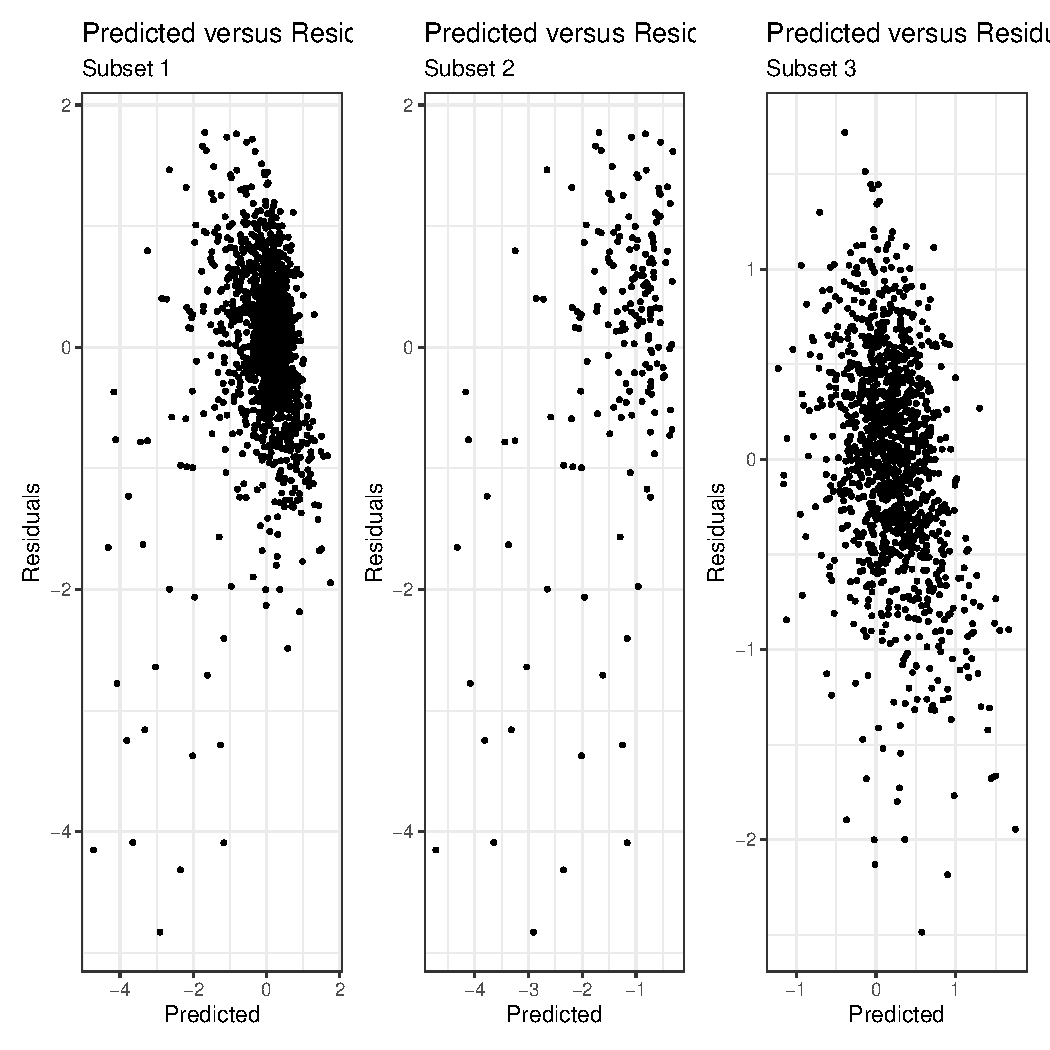
\includegraphics[width=\maxwidth]{figure/unnamed-chunk-13-4} 
\begin{kframe}\begin{alltt}
\hlkwd{predictForSubsets}\hlstd{(model.2.accur,} \hlstr{"WeightLogSC"}\hlstd{,}
                  \hlstd{births,}
                  \hlstd{births} \hlopt \hlkwd{filter}\hlstd{(Premie}\hlopt{==}\hlstr{"Yes"}\hlstd{),}
                  \hlstd{births} \hlopt \hlkwd{filter}\hlstd{(Premie}\hlopt{==}\hlstr{"No"}\hlstd{))}
\end{alltt}
\begin{verbatim}
## [1] "Subset 1 R-Squared: 0.524330514867102"
## [1] "Subset 1 Mean Abs. Error: 0.493034075135682"
\end{verbatim}
\end{kframe}
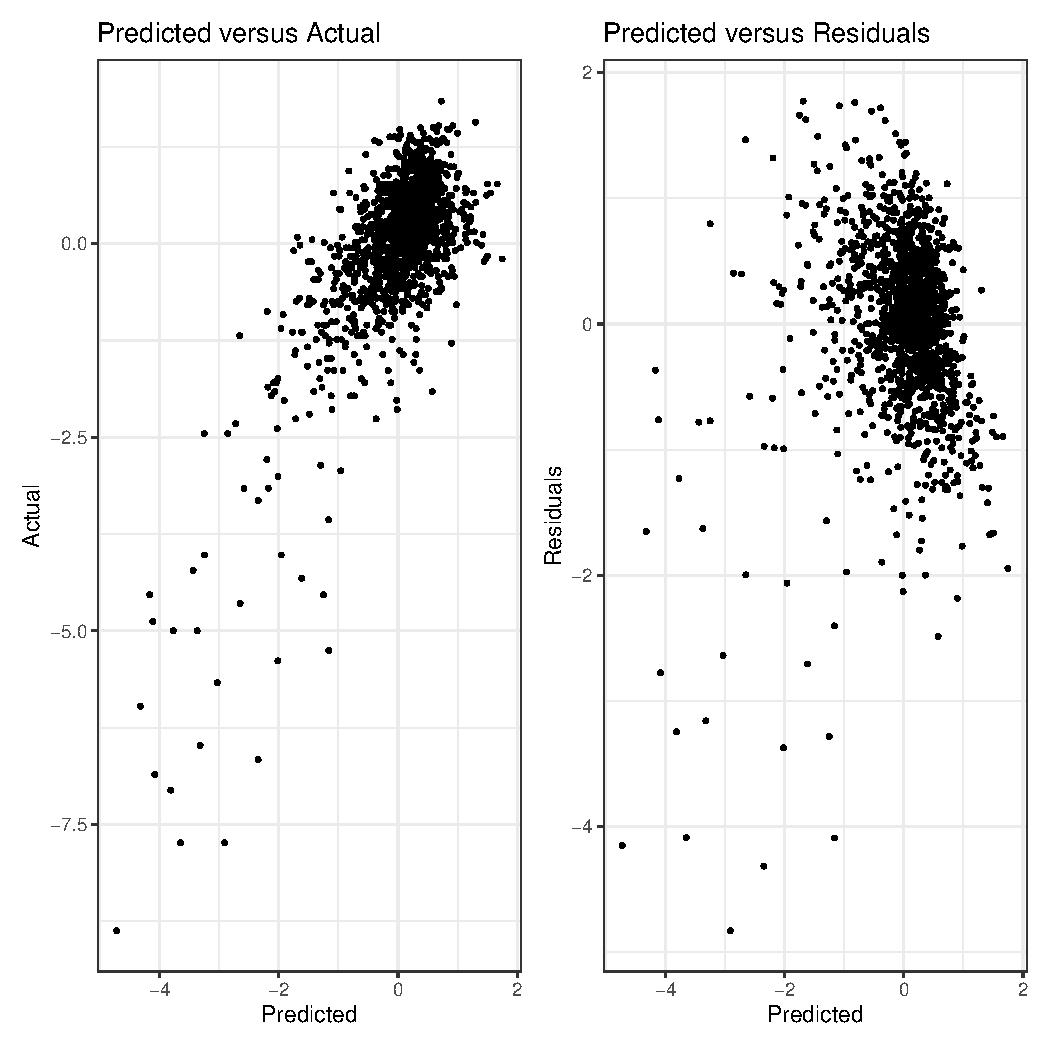
\includegraphics[width=\maxwidth]{figure/unnamed-chunk-13-5} 
\begin{kframe}\begin{verbatim}
## [1] "Subset 2 R-Squared: 0.655114101459069"
## [1] "Subset 2 Mean Abs. Error: 0.884841254580077"
\end{verbatim}
\end{kframe}
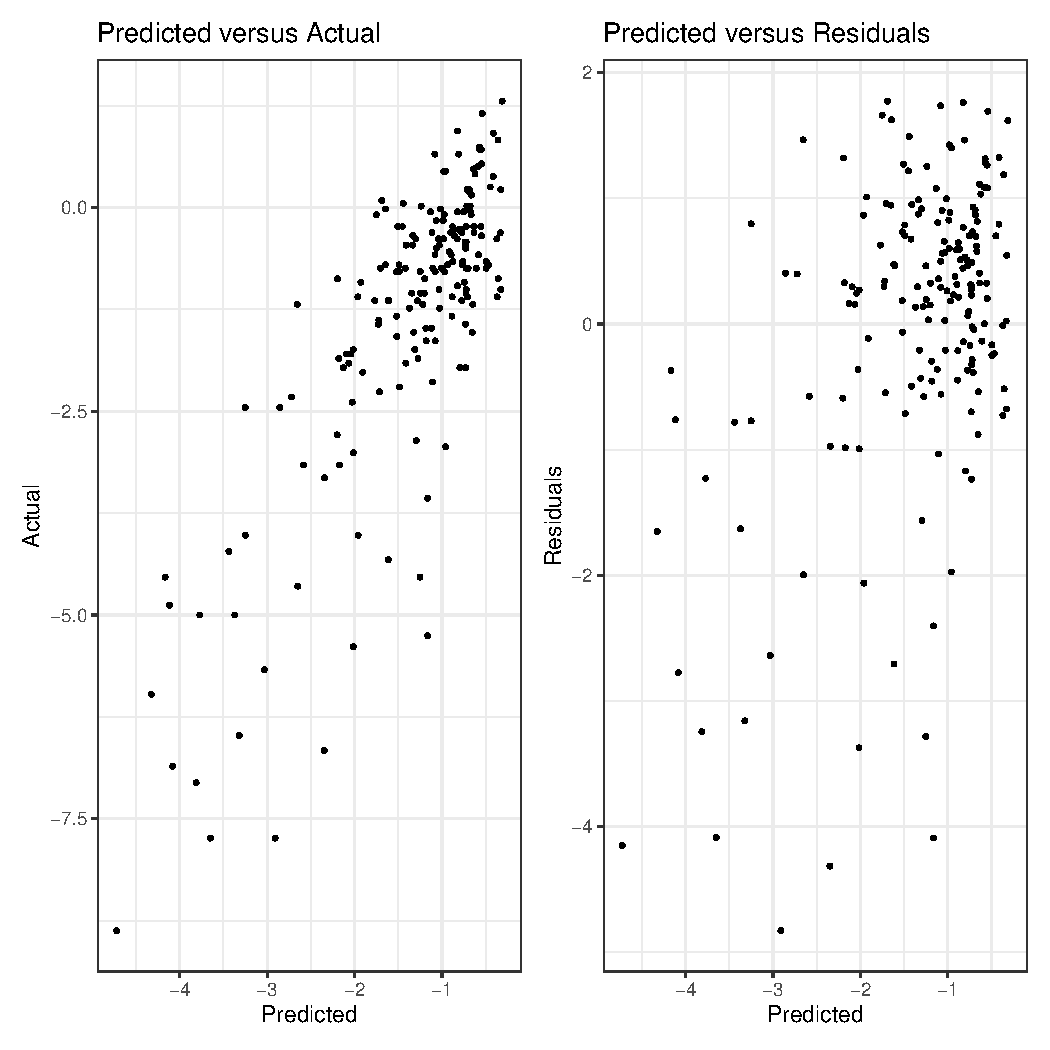
\includegraphics[width=\maxwidth]{figure/unnamed-chunk-13-6} 
\begin{kframe}\begin{verbatim}
## [1] "Subset 3 R-Squared: 0.153089471782906"
## [1] "Subset 3 Mean Abs. Error: 0.435283994126369"
\end{verbatim}
\end{kframe}
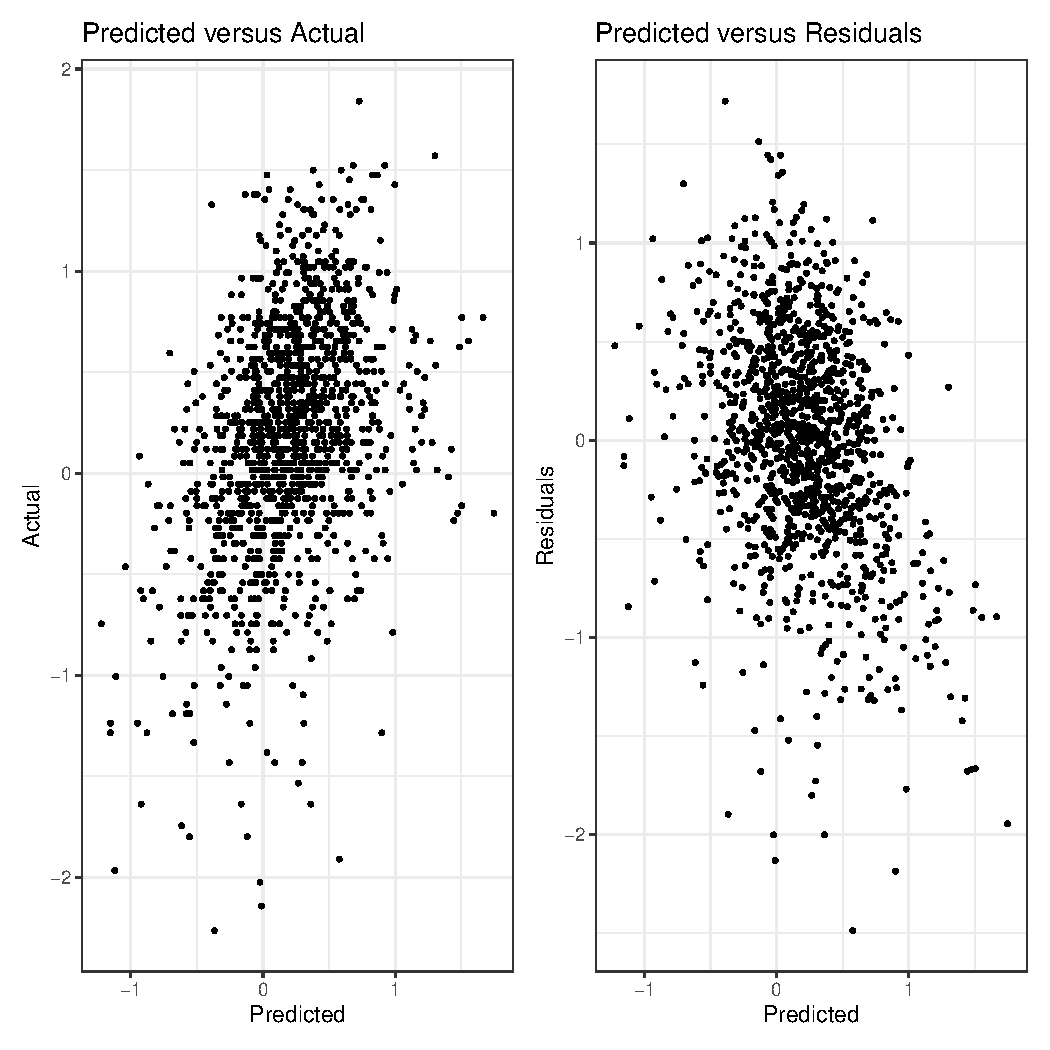
\includegraphics[width=\maxwidth]{figure/unnamed-chunk-13-7} 
\end{knitrout}


\begin{table}[ht]
\centering
\begin{tabular}{lrrr}
  \hline
  Subset & R-Squared & Mean Absolute Error\\ 
  \hline
   Births & 0.4570 & 0.5714 \\ 
   Preemies & 0.5510 & 0.7090 \\ 
   Not Preemies & 0.1755 & 0.5511 \\
   \hline
\end{tabular}
\caption{Summary of all adjusted first order regression model R-squared, Adj R-squared, RSE, AIC, and BIC.}
\end{table}


Part 2: AIC/BIC Iteration 1
\begin{knitrout}
\definecolor{shadecolor}{rgb}{0.969, 0.969, 0.969}\color{fgcolor}\begin{kframe}
\begin{alltt}
\hlcom{## Assumptions Model}

\hlstd{x} \hlkwb{<-} \hlkwd{model.matrix}\hlstd{(model.2.assu)[,}\hlopt{-}\hlnum{1}\hlstd{]}

\hlstd{y} \hlkwb{<-} \hlstd{births}\hlopt{$}\hlstd{WeightGmSC}

\hlstd{xy} \hlkwb{<-} \hlkwd{as.data.frame}\hlstd{(}\hlkwd{cbind}\hlstd{(x,y))}
\hlstd{best.subsets.aic} \hlkwb{<-} \hlkwd{bestglm}\hlstd{(xy,} \hlkwc{IC}\hlstd{=}\hlstr{"AIC"}\hlstd{,} \hlkwc{TopModels} \hlstd{=} \hlnum{5}\hlstd{)}
\hlstd{best.model.aic} \hlkwb{<-} \hlstd{best.subsets.aic}\hlopt{$}\hlstd{BestModel}
\hlkwd{modelSummary}\hlstd{(best.model.aic)}
\end{alltt}
\begin{verbatim}
##                    Estimate Std. Error   t value     Pr(>|t|)
## (Intercept)       0.1155533 0.03565298  3.241056 0.0012189440
## Plural2          -1.1195941 0.12177905 -9.193651 0.0000000000
## Plural3          -1.4808912 0.37795193 -3.918200 0.0000935265
## SexMale           0.1502685 0.03951570  3.802753 0.0001492650
## MomAgeSC          0.1054359 0.02244925  4.696635 0.0000029051
## WeeksSC           0.4196465 0.02914455 14.398801 0.0000000000
## RaceMomBlack     -0.1665708 0.05073699 -3.283025 0.0010523894
## RaceMomFilipino  -1.4157231 0.74133018 -1.909706 0.0563756484
## MaritalUnmarried -0.0790069 0.05003876 -1.578914 0.1145821349
## GainedSC          0.1737710 0.01995059  8.710069 0.0000000000
## SmokeYes         -0.3216242 0.05699092 -5.643428 0.0000000202
## PremieYes        -0.3511604 0.08474998 -4.143486 0.0000362603
## [1] "R-squared: 0.456717769215429"
## [1] "Adjusted R-Squared: 0.452439956374606"
## [1] "Sigma: 0.739973001957095"
## [1] "AIC: 3163.90042969188"
## [1] "BIC: 3232.15869134656"
## [1] "Quantile Departure: 0.0474199906966593"
\end{verbatim}
\end{kframe}
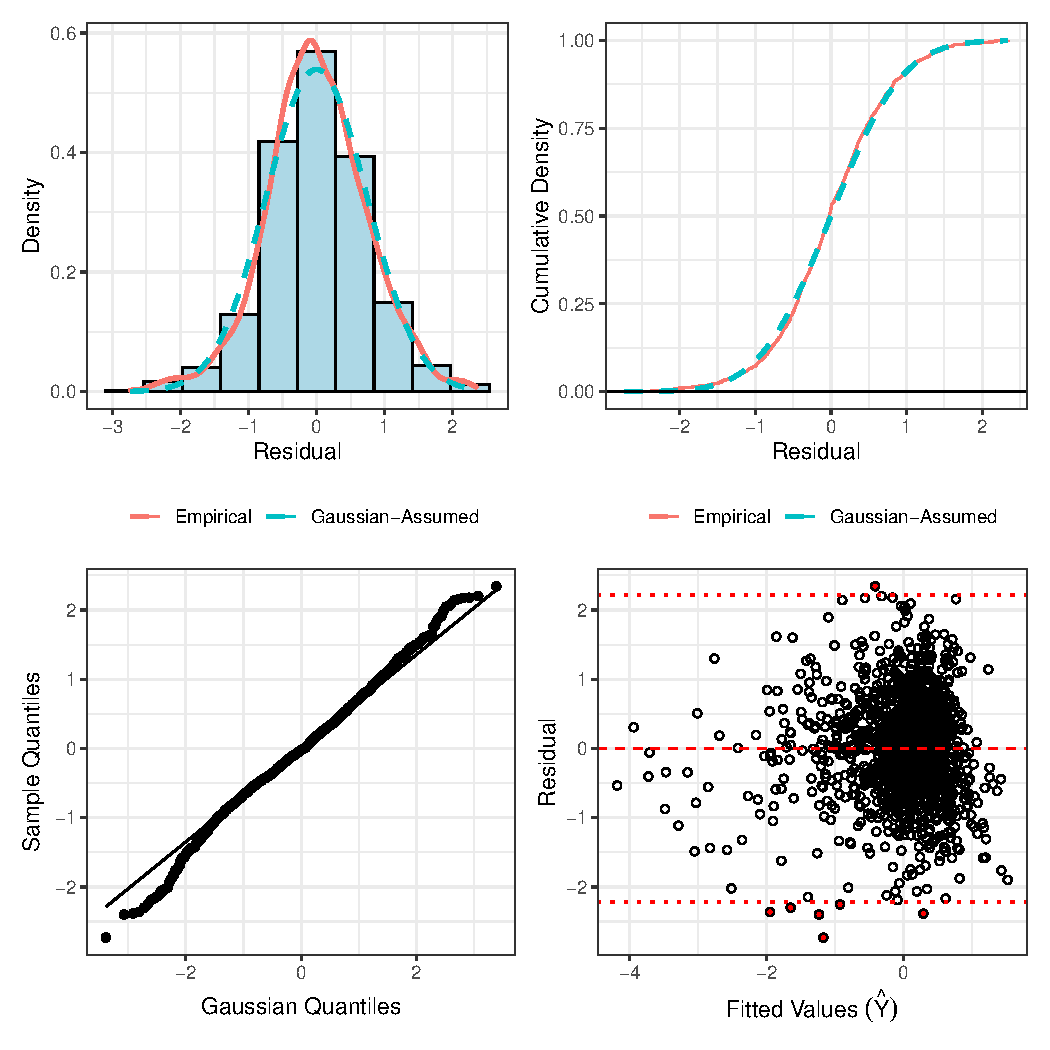
\includegraphics[width=\maxwidth]{figure/unnamed-chunk-14-1} 
\begin{kframe}\begin{alltt}
\hlstd{best.subsets.bic} \hlkwb{<-} \hlkwd{bestglm}\hlstd{(xy,} \hlkwc{IC}\hlstd{=}\hlstr{"BIC"}\hlstd{,} \hlkwc{TopModels} \hlstd{=} \hlnum{5}\hlstd{)}
\hlstd{best.model.bic} \hlkwb{<-} \hlstd{best.subsets.bic}\hlopt{$}\hlstd{BestModel}
\hlkwd{modelSummary}\hlstd{(best.model.bic)}
\end{alltt}
\begin{verbatim}
##                 Estimate Std. Error   t value     Pr(>|t|)
## (Intercept)   0.09475252 0.03368651  2.812773 0.0049802705
## Plural2      -1.12009473 0.12195379 -9.184583 0.0000000000
## Plural3      -1.47212718 0.37849237 -3.889450 0.0001051871
## SexMale       0.15216134 0.03956124  3.846223 0.0001253459
## MomAgeSC      0.11860642 0.02041483  5.809816 0.0000000077
## WeeksSC       0.41869752 0.02918503 14.346313 0.0000000000
## RaceMomBlack -0.19170667 0.04813574 -3.982627 0.0000716623
## GainedSC      0.17381907 0.01997972  8.699777 0.0000000000
## SmokeYes     -0.33430893 0.05643831 -5.923439 0.0000000040
## PremieYes    -0.35772800 0.08478370 -4.219302 0.0000260829
## [1] "R-squared: 0.45431789056999"
## [1] "Adjusted R-Squared: 0.450807426678017"
## [1] "Sigma: 0.741075281818239"
## [1] "AIC: 3166.11079739794"
## [1] "BIC: 3223.86778802883"
## [1] "Quantile Departure: 0.0461987895225344"
\end{verbatim}
\end{kframe}
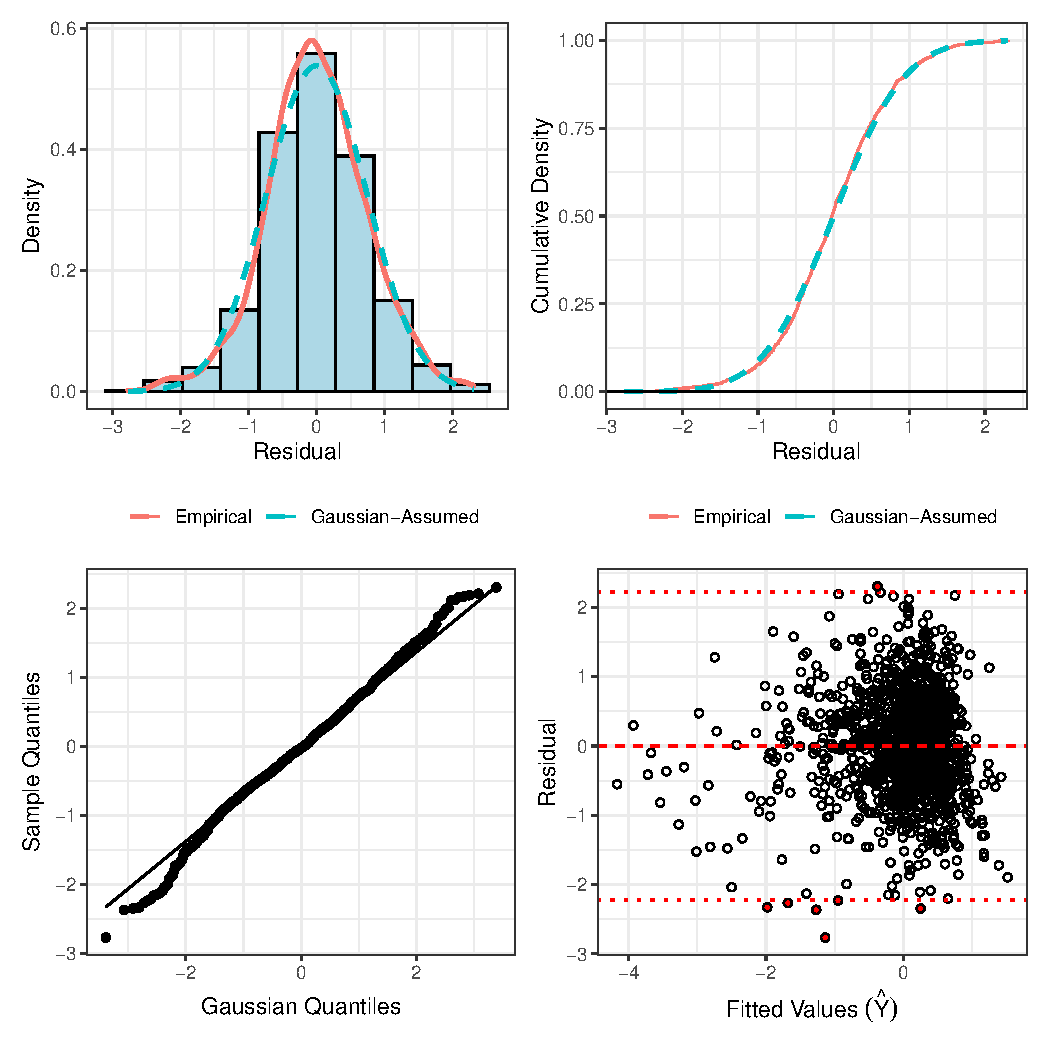
\includegraphics[width=\maxwidth]{figure/unnamed-chunk-14-2} 
\begin{kframe}\begin{alltt}
\hlstd{regsubsets.out} \hlkwb{<-} \hlkwd{regsubsets}\hlstd{(WeightGmSC} \hlopt{~} \hlstd{Plural} \hlopt{+} \hlstd{Sex} \hlopt{+} \hlstd{MomAgeSC} \hlopt{+} \hlstd{WeeksSC} \hlopt{+} \hlstd{RaceMom} \hlopt{+}
                               \hlstd{Marital} \hlopt{+} \hlstd{GainedSC} \hlopt{+} \hlstd{Smoke} \hlopt{+} \hlstd{Premie,}
                             \hlkwc{data}\hlstd{=births,} \hlkwc{nbest} \hlstd{=} \hlnum{1}\hlstd{,} \hlkwc{nvmax}\hlstd{=}\hlnum{15}\hlstd{)}

\hlkwd{as.data.frame}\hlstd{(}\hlkwd{summary}\hlstd{(regsubsets.out)}\hlopt{$}\hlstd{outmat)}
\end{alltt}
\begin{verbatim}
##           Plural2 Plural3 SexMale MomAgeSC WeeksSC RaceMomBlack RaceMomChinese
## 1  ( 1 )                                         *                            
## 2  ( 1 )                                         *                            
## 3  ( 1 )        *                                *                            
## 4  ( 1 )        *                        *       *                            
## 5  ( 1 )        *                        *       *                            
## 6  ( 1 )        *                        *       *                            
## 7  ( 1 )        *                        *       *            *               
## 8  ( 1 )        *       *                *       *            *               
## 9  ( 1 )        *       *       *        *       *            *               
## 10  ( 1 )       *       *       *        *       *            *               
## 11  ( 1 )       *       *       *        *       *            *               
## 12  ( 1 )       *       *       *        *       *            *               
## 13  ( 1 )       *       *       *        *       *            *              *
## 14  ( 1 )       *       *       *        *       *            *               
## 15  ( 1 )       *       *       *        *       *            *              *
##           RaceMomFilipino RaceMomJapanese RaceMomOther Asian / PI RaceMomWhite
## 1  ( 1 )                                                                      
## 2  ( 1 )                                                                      
## 3  ( 1 )                                                                      
## 4  ( 1 )                                                                      
## 5  ( 1 )                                                                      
## 6  ( 1 )                                                                      
## 7  ( 1 )                                                                      
## 8  ( 1 )                                                                      
## 9  ( 1 )                                                                      
## 10  ( 1 )               *                                                     
## 11  ( 1 )               *                                                     
## 12  ( 1 )               *                                       *             
## 13  ( 1 )               *                                       *             
## 14  ( 1 )               *               *                       *            *
## 15  ( 1 )               *               *                       *            *
##           MaritalUnmarried GainedSC SmokeYes PremieYes
## 1  ( 1 )                                              
## 2  ( 1 )                          *                   
## 3  ( 1 )                          *                   
## 4  ( 1 )                          *                   
## 5  ( 1 )                          *        *          
## 6  ( 1 )                          *        *         *
## 7  ( 1 )                          *        *         *
## 8  ( 1 )                          *        *         *
## 9  ( 1 )                          *        *         *
## 10  ( 1 )                         *        *         *
## 11  ( 1 )                *        *        *         *
## 12  ( 1 )                *        *        *         *
## 13  ( 1 )                *        *        *         *
## 14  ( 1 )                *        *        *         *
## 15  ( 1 )                *        *        *         *
\end{verbatim}
\begin{alltt}
\hlstd{fit.stats} \hlkwb{<-} \hlkwd{data.frame}\hlstd{(}\hlkwc{num.variables}\hlstd{=}\hlnum{1}\hlopt{:}\hlnum{15}\hlstd{,}
                        \hlkwc{adjr2} \hlstd{=} \hlkwd{summary}\hlstd{(regsubsets.out)}\hlopt{$}\hlstd{adjr2,}
                        \hlkwc{bic}\hlstd{=}\hlkwd{summary}\hlstd{(regsubsets.out)}\hlopt{$}\hlstd{bic)}
\hlstd{fit.stats}
\end{alltt}
\begin{verbatim}
##    num.variables     adjr2       bic
## 1              1 0.3419165 -576.0584
## 2              2 0.3659468 -622.2229
## 3              3 0.3936644 -678.9560
## 4              4 0.4139286 -720.6032
## 5              5 0.4262316 -744.2497
## 6              6 0.4342432 -757.8164
## 7              7 0.4397681 -765.3984
## 8              8 0.4453965 -773.3810
## 9              9 0.4508074 -780.9513
## 10            10 0.4518552 -777.3989
## 11            11 0.4524400 -772.6604
## 12            12 0.4523523 -766.1931
## 13            13 0.4519692 -758.9668
## 14            14 0.4515905 -751.7534
## 15            15 0.4512188 -744.5593
\end{verbatim}
\begin{alltt}
\hlcom{## Of the models, BIC suggests removing Marital and all races}
\hlcom{## except Black. AIC / radj2 would retain Filipino and Marital.}
\hlcom{## Since there is only a single Philipino instance, we remove Filipino,}
\hlcom{## as well as marital since the significance is so low.}
\end{alltt}
\end{kframe}
\end{knitrout}

\section{Part 5: Final Model(s) and Conclusions.}
\begin{knitrout}
\definecolor{shadecolor}{rgb}{0.969, 0.969, 0.969}\color{fgcolor}\begin{kframe}
\begin{alltt}
\hlstd{assessModel} \hlkwb{<-} \hlkwa{function}\hlstd{(}\hlkwc{model}\hlstd{) \{}
  \hlkwd{print}\hlstd{(}\hlkwd{modelSummary}\hlstd{(model))}
  \hlkwd{print}\hlstd{(}\hlkwd{vif}\hlstd{(model))}
  \hlkwd{print}\hlstd{(}\hlkwd{summary}\hlstd{(model}\hlopt{$}\hlstd{residual))}
  \hlkwd{print}\hlstd{(}\hlkwd{confint}\hlstd{(model))}
  \hlstd{lev} \hlkwb{<-} \hlstd{model}\hlopt{$}\hlstd{model} \hlopt \hlkwd{mutate}\hlstd{(}\hlkwc{h.values} \hlstd{=} \hlkwd{hatvalues}\hlstd{(model))}
  \hlkwd{print}\hlstd{(}\hlkwd{summary}\hlstd{(lev}\hlopt{$}\hlstd{h.values))}
  \hlstd{p} \hlkwb{<-} \hlnum{2}
  \hlstd{n} \hlkwb{<-} \hlkwd{nrow}\hlstd{(model}\hlopt{$}\hlstd{model)}
  \hlstd{high.lev} \hlkwb{<-} \hlstd{lev} \hlopt \hlkwd{filter}\hlstd{(h.values} \hlopt{>} \hlnum{2}\hlopt{*}\hlstd{p}\hlopt{/}\hlstd{n)}
  \hlkwd{print}\hlstd{(}\hlkwd{paste}\hlstd{(}\hlstr{"High Lev.:"}\hlstd{,} \hlkwd{nrow}\hlstd{(high.lev)))}
  \hlstd{v.high.lev} \hlkwb{<-} \hlstd{lev} \hlopt \hlkwd{filter}\hlstd{(h.values} \hlopt{>} \hlnum{3}\hlopt{*}\hlstd{p}\hlopt{/}\hlstd{n)}
  \hlkwd{print}\hlstd{(}\hlkwd{paste}\hlstd{(}\hlstr{"Very High Lev.:"}\hlstd{,} \hlkwd{nrow}\hlstd{(v.high.lev)))}
  \hlstd{new.resid} \hlkwb{<-} \hlstd{model}\hlopt{$}\hlstd{model} \hlopt \hlkwd{mutate}\hlstd{(}\hlkwc{stdres} \hlstd{=} \hlkwd{rstandard}\hlstd{(model),}
                                      \hlkwc{stures} \hlstd{=} \hlkwd{rstudent}\hlstd{(model))}
  \hlkwd{print}\hlstd{(}\hlstr{"Standard Residual Quant.:"}\hlstd{)}
  \hlkwd{print}\hlstd{(}\hlkwd{summary}\hlstd{(new.resid}\hlopt{$}\hlstd{stdres))}
  \hlkwd{print}\hlstd{(}\hlstr{"Studentized Residual Quant.:"}\hlstd{)}
  \hlkwd{print}\hlstd{(}\hlkwd{summary}\hlstd{(new.resid}\hlopt{$}\hlstd{stures))}
  \hlstd{s.outliers.stdres} \hlkwb{<-} \hlstd{new.resid} \hlopt \hlkwd{filter}\hlstd{(}\hlkwd{abs}\hlstd{(stdres)}\hlopt{>}\hlnum{3}\hlstd{)}
  \hlkwd{print}\hlstd{(}\hlkwd{paste}\hlstd{(}\hlstr{"Strong Standard Residual Outliers:"}\hlstd{,} \hlkwd{nrow}\hlstd{(s.outliers.stdres)))}
  \hlkwd{print}\hlstd{(s.outliers.stdres)}
  \hlstd{s.outliers.stures} \hlkwb{<-} \hlstd{new.resid} \hlopt \hlkwd{filter}\hlstd{(}\hlkwd{abs}\hlstd{(stures)}\hlopt{>}\hlnum{3}\hlstd{)}
  \hlkwd{print}\hlstd{(}\hlkwd{paste}\hlstd{(}\hlstr{"String Studentized Residual Outliers:"}\hlstd{,} \hlkwd{nrow}\hlstd{(s.outliers.stures)))}
  \hlkwd{print}\hlstd{(s.outliers.stures)}
  \hlstd{cooks.values} \hlkwb{<-} \hlstd{model}\hlopt{$}\hlstd{model} \hlopt \hlkwd{mutate}\hlstd{(}\hlkwc{cooks} \hlstd{=} \hlkwd{cooks.distance}\hlstd{(model))}
  \hlkwd{print}\hlstd{(}\hlstr{"Cook's Values:"}\hlstd{)}
  \hlkwd{print}\hlstd{(}\hlkwd{summary}\hlstd{(cooks.values}\hlopt{$}\hlstd{cooks))}
  \hlstd{cooks.strong} \hlkwb{<-} \hlstd{cooks.values} \hlopt \hlkwd{filter}\hlstd{(cooks}\hlopt{>}\hlnum{1}\hlstd{)}
  \hlkwd{print}\hlstd{(}\hlkwd{paste}\hlstd{(}\hlstr{"Strong C. Values:"}\hlstd{,} \hlkwd{nrow}\hlstd{(cooks.strong)))}
\hlstd{\}}

\hlkwd{assessModel}\hlstd{(mod.accur.final)}
\end{alltt}


{\ttfamily\noindent\bfseries\color{errorcolor}{\#\# Error in summary(model): object 'mod.accur.final' not found}}\begin{alltt}
\hlkwd{assessModel}\hlstd{(mod.accur.final.part)}
\end{alltt}


{\ttfamily\noindent\bfseries\color{errorcolor}{\#\# Error in summary(model): object 'mod.accur.final.part' not found}}\begin{alltt}
\hlkwd{assessModel}\hlstd{(min.vif.model)}
\end{alltt}


{\ttfamily\noindent\bfseries\color{errorcolor}{\#\# Error in summary(model): object 'min.vif.model' not found}}\end{kframe}
\end{knitrout}


Highest Accuracy Model:
\begin{align*} 
\hat{y} &= 0.119 + -1.165\cdot \text{I}(\text{Plural} = 2) + -2.006\cdot \text{I}(\text{Plural} = 3) + 0.104\cdot \text{I}(\text{Sex} = \text{Male}) \newline &\quad + 0.110\cdot \text{MomAgeSC} + 0.398\cdot \text{WeeksSC} - 0.272\cdot \text{I}(\text{Black} = \text{TRUE}) + 0.150\cdot \text{GainedSC} \newline &\quad -0.303\cdot \text{I}(\text{Smoke} = \text{Yes}) - 0.393\cdot \text{I}(\text{Premie} = \text{Yes}) - 0.098\cdot \text{MomAgeSC} \cdot \text{I}(\text{Smoke} = \text{Yes}) \newline &\quad + 0.366\cdot \text{WeeksSC} \cdot \text{I}(\text{Black} = \text{TRUE}) - 0.153\cdot \text{WeeksSC} \cdot \text{GainedSC} - 0.037\cdot \text{WeeksSC} \cdot \text{I}(\text{Smoke} = \text{Yes}) \newline &\quad + 0.202\cdot \text{I}(\text{Black} = \text{TRUE}) \cdot \text{I}(\text{Smoke} = \text{Yes}) + 0.781\cdot \text{I}(\text{Black} = \text{TRUE}) \cdot \text{I}(\text{Premie} = \text{Yes}) \end{align*}


Highest accuracy with the slowest departure from Minimizing residuals:
\begin{align*} 
\hat{y} &= 0.1122 + -1.2928 \cdot \text{I}(\text{Plural} = 2) + -0.7222 \cdot \text{I}(\text{Plural} = 3) + 0.1476 \cdot \text{I}(\text{Sex} = \text{Male}) \newline &\quad + 0.1653 \cdot \text{MomAgeSC} - 0.0259 \cdot \text{MomAgeSq} + 0.4193 \cdot \text{WeeksSC} - 0.2278 \cdot \text{I}(\text{Black} = \text{TRUE}) \newline &\quad + 0.1291 \cdot \text{GainedSC} + 0.0473 \cdot \text{GainedSq} - 0.3935 \cdot \text{I}(\text{Smoke} = \text{Yes}) - 0.2733 \cdot \text{I}(\text{Premie} = \text{Yes}) \newline &\quad - 0.0698 \cdot \text{I}(\text{Plural} = 2) \cdot \text{WeeksSC} + 0.2816 \cdot \text{I}(\text{Plural} = 3) \cdot \text{WeeksSC} - 0.0232 \cdot \text{MomAgeSC} \cdot \text{MomAgeSq} \newline &\quad -0.0237 \cdot \text{MomAgeSC} \cdot \text{WeeksSC} + 0.0304 \cdot \text{MomAgeSC} \cdot \text{GainedSq} - 0.1097 \cdot \text{MomAgeSC} \cdot \text{I}(\text{Smoke} = \text{Yes}) \newline &\quad - 0.0683 \cdot \text{MomAgeSq} \cdot \text{I}(\text{Black} = \text{TRUE}) + 0.0401 \cdot \text{MomAgeSq} \cdot \text{GainedSC} \newline &\quad - 0.0260 \cdot \text{WeeksSC} \cdot \text{I}(\text{Smoke} = \text{Yes}) + 0.2425 \cdot \text{WeeksSC} \cdot \text{I}(\text{Black} = \text{TRUE}) \newline &\quad - 0.0703 \cdot \text{GainedSq} \cdot \text{I}(\text{Smoke} = \text{Yes}) - 0.2656 \cdot \text{GainedSq} \cdot \text{I}(\text{Premie} = \text{Yes}) \newline &\quad +-0.2656 \cdot \text{GainedSq} \cdot \text{I}(\text{Premie} = \text{Yes}) + 0.2978 \cdot \text{I}(\text{Black} = \text{TRUE}) \cdot \text{I}(\text{Smoke} = \text{Yes}) \newline &\quad + 0.6522 \cdot \text{I}(\text{Black} = \text{TRUE}) \cdot \text{I}(\text{Premie} = \text{Yes}) 
\end{align*}

max accuracy with limited variables
\begin{align*} 
\hat{y} &= 0.1726 + -1.1681\cdot \text{I}(\text{Plural} = 2) + -0.9379\cdot \text{I}(\text{Plural} = 3) + -0.1535\cdot \text{I}(\text{Black} = \text{TRUE}) \newline &\quad + 0.9901\cdot \text{I}(\text{Premie} = \text{Yes}) + 0.1172\cdot \text{I}(\text{Sex} = \text{Male}) + 0.0793\cdot \text{MomAgeSC} + 0.1775\cdot \text{WeeksSC} \newline &\quad + 0.1245\cdot \text{GainedSC} - 0.3038\cdot \text{I}(\text{Smoke} = \text{Yes}) - 0.2830\cdot \text{I}(\text{Plural} = 2)\cdot \text{WeeksSC} - 0.1058\cdot \text{I}(\text{Plural} = 3)\cdot \text{WeeksSC} \newline &\quad + 0.1665\cdot \text{I}(\text{Black} = \text{TRUE})\cdot \text{I}(\text{Smoke} = \text{Yes}) + 1.1655\cdot \text{I}(\text{Premie} = \text{Yes})\cdot \text{WeeksSC} + 0.3570\cdot \text{I}(\text{Premie} = \text{Yes})\cdot \text{I}(\text{Smoke} = \text{Yes}) 
\end{align*}


\end{document}
